%&pdflatex
%!TEX TS-program = pdflatex
%!TEX encoding = UTF-8 Unicode

\documentclass[11pt]{book}

%--------------------------------------------------------------------------- 
% Paquetes y fuentes
%---------------------------------------------------------------------------

% Definir un nuevo comando para la B caligráfica
\newcommand{\BD}{\text{$\mathcal{B}\mathcal{D}$}}

\usepackage{geometry}               % define las dimensiones de la página
\geometry{
 a4paper, % Tamaño del papel
 centering, % Zona útil centrada
 margin = 25mm, % Márgenes en blanco: 25mm
}

\usepackage[utf8]{inputenc}        % para usar el teclado normalmente
\usepackage[spanish,es-tabla]{babel}        % idioma español
\usepackage[T1]{fontenc}           % gestión de fuentes con acentos
\usepackage{csquotes}              % citas (necesario con biblatex)

% Matemáticas y teoremas
\usepackage{amssymb}               
\usepackage{amsmath}               
\usepackage{amsthm}                
\usepackage{mathptmx}              % fuente Times

% Gráficos y figuras
\usepackage{tikz}                  
\usepackage{pgfplots}
\pgfplotsset{compat=1.17}
%\usepackage[draft]{graphicx}       % draft = no carga imágenes al compilar

% Código y algoritmos
\usepackage{listings}
\usepackage[ruled,vlined,spanish,onelanguage]{algorithm2e}
\SetKw{Para}{Para}

% Color portada
\usepackage{xcolor}
\definecolor{miRojo}{HTML}{BA0C2F}

% Hipervínculos
\usepackage[colorlinks=true, allcolors=blue]{hyperref}

% Tipografía
\usepackage{microtype}

% Cabeceras y pies de página
\usepackage{titleps}

% Bibliografía
\usepackage[style=apa,backend=biber]{biblatex}
\DeclareLanguageMapping{spanish}{spanish-apa}
\addbibresource{refs.bib}

% Referencias cruzadas inteligentes
\usepackage{cleveref}

% Tabla 
\usepackage{booktabs} % Para líneas más elegantes en la tabla
\usepackage{siunitx}

%--------------------------------------------------------------------------- 
% Definición de estilos de página
%---------------------------------------------------------------------------

\newpagestyle{miestilo}{
\sethead[\thepage][][\textsl{\chaptername\ \thechapter. \chaptertitle}]
{\textsl{Transfomer pequeño para generación de texto \ - \ Diego García Muro}}{}{\thepage}
}

\newpagestyle{primeraparte}{
\sethead[\thepage][][\textsl{\chaptertitle}]
{\textsl{Transfomer pequeño para generación de texto \ - \ Diego García Muro}}{}{\thepage}
}

\newcommand{\clearemptydoublepage}{\newpage{\pagestyle{empty}\cleardoublepage}}
\newcommand{\sectionmarkwithoutsections}[1]{\markright{#1}}

\makeindex

%--------------------------------------------------------------------------- 
% Definición de entornos tipo teorema
%---------------------------------------------------------------------------

\theoremstyle{plain}
\newtheorem{teorema}{Teorema}[chapter]
\newtheorem{prop}[teorema]{Proposición}
\newtheorem{corolario}[teorema]{Corolario}
\newtheorem{lema}[teorema]{Lema}

\theoremstyle{definition}
\newtheorem*{defin}{Definición}
\newtheorem{ejemplo}{Ejemplo}
\newtheorem{nota}{Nota}[chapter]

%--------------------------------------------------------------------------- 
% Atajos matemáticos
%---------------------------------------------------------------------------

\newcommand\N{\mathbb{N}}
\newcommand\Z{\mathbb{Z}}
\newcommand\R{\mathbb{R}}
\newcommand\C{\mathbb{C}}

\renewcommand{\spanishoperators}{Re}

%--------------------------------------------------------------------------- 
% Inicio del documento
%---------------------------------------------------------------------------

\begin{document}
\frontmatter
\pagestyle{primeraparte}


%\pagenumbering{roman} % Incluido en \frontmatter


%--- PORTADA DEL TFG
\begin{titlepage}
    \centering

    \begin{figure}
    \centering
    
\includegraphics[width=0.25\linewidth]{img/logo_imf.png}
    \end{figure}

    \vspace*{1cm}
    {\Large \textbf{MÁSTER EN} \\[0.3cm]
    \textbf{Big Data e Inteligencia Artificial} \\[1cm]
    \textbf{ONLINE}}\\[3cm]
    
    {\LARGE \textcolor{miRojo}{\textbf{Implementación de una arquitectura Transformer educativa (NLP).}}} \\[2cm]
    
    {\large TFM elaborado por: \\[0.3cm]
    \textbf{Diego García Muro}} \\[1cm]
    
    {\large Tutor/a de TFM: \\[0.3cm]
    \textbf{Daniel Rubio Yagüe}} \\[4cm]
    
    {\large - Soria, 16 Septiembre del 2025 - }
    
    \vfill
\end{titlepage}
%--- FIN DE LA PORTADA

\clearemptydoublepage


%--- RESUMEN

\chapter{Resumen}
 Explicación de la arquitectura Transformer, importancia y lo que contiene el documento
%--- FIN DEL RESUMEN

\clearemptydoublepage

\chapter{Abstract}
 Lo mismo pero en inglés
\clearemptydoublepage

\tableofcontents

\clearemptydoublepage

%-------------
\mainmatter                      % Parte principal del texto
\pagestyle{miestilo}    % Estilo de cabeceras para la parte principal del texto

%--- CAPÍTULO 1 DEL TFM
\chapter{Introducción y antecedentes}
En los últimos años, el auge de la inteligencia artificial ha estado impulsado por los llamados Large Language Models (LLMs), que han supuesto una revolución, transformando sectores enteros. Estos modelos están presentes tanto como herramientas que poco a poco reemplazan a los buscadores tradicionales, usadas por el público en general, como herramientas open source o de pago por uso, accesibles localmente o a través de la nube, que han dado un giro al negocio en general, originando nuevas oportunidades, automatizando tareas y ofreciendo soluciones a problemas que, o no existían o no se podían abordar con tanta efectividad.


Este tipo de modelos se construyen haciendo uso de enormes recursos computacionales y pueden llegar a tener billones de parámetros, lo que dificulta enormemente su implementación. Es por ello, que en este anteproyecto se propone el desarrollo de un modelo reducido basado en la arquitectura Transformer, con un número reducido de parámetros capaz de entrenarse usando una GPU de propósito
general en unas horas. El objetivo principal no es competir con modelos de última generación, sino comprender los fundamentos teóricos y prácticos de los Transformers y explorar, de manera didáctica, su funcionamiento en tareas de procesamiento de lenguaje natural.

\section{De modelos secuenciales a mecanismos de atención}
Antes de la aparición de esta arquitectura, los modelos existentes procesaban las palabras de forma secuencial con el fin de entender el lenguaje. Esto implica una complejidad [O(n²)] de forma que para procesar 3 palabras se tenían que ejecutar 6 operaciones secuenciales (para la tercera palabra necesita recordar la primera y segunda y procesar la tercera, para la segunda tendría que recordar la primera y procesar la segunda y para la primera se debía procesar esa palabra), esto, para 10 palabras aumenta a 45 operaciones, y para 100, 4950. Computacionalmente es muy ineficiente. 

Gracias al paper \textit{"Attention is ALl you Need"} publicado en 2017 \parencite{vaswani2017attention}, donde se presentan los \textit{mecanismos de atención} y se logra optimizar el proceso a una complejidad [O(n)]. Esto es porque plantean la posibilidad de que cada palabra mire simultáneamente a las demás, es decir, ya no hay un procesamiento secuencial, sino paralelo. 

Estos mecanismos constan de 8 operaciones. En primer lugar trabajan con \textit{embeddings} \parencite{neuraforge2023guide}, esto es, vectores densos que recogen, tras el entrenamiento, información sobre cada token en relación con el resto, ya sea información semántica, relaciones sintácticas, etc. Estas representaciones, se proyectan a 3 matrices, también entrenables, que son la base de los mecanismos de atención: Q (¿Qué busco?), K (¿Qué aporto?), V (La información real aportada) \parencite{epichka2023qkv}. A partir de ellas, se calcula una métrica de atención, que indicaría para cada token o palabra, como de relevante es. Esta métrica se convierte a una distribución de probabilidad a través de la función \textit{softmax}, de forma que simula una conciencia humana, pues los seres humanos nos enfocamos en aquella información relevante mientras que el resto queda en la periferia. Por último, se integra la información, dando a la información real (V) un peso, dado por esos pesos de atención calculados previamente.

Todo este proceso no se ejecuta una única vez, sino que se apila en capas, de forma que cada capa o cabeza de atención se encarga de una tarea distinta. Así, las capas más superficiales capturan relaciones sintácticas del tipo sujeto-verbo-objeto, mientras que las capas más profundas abordan el razonamiento abstracto y el procesamiento meta-cognitivo, de hecho, se cree que en las capas 70 a 80 de los modelos GPT la representación se asemeja al comportamiento humano \parencite{plainenglish2021gpt}. En este punto, un elemento clave es el \textit{flujo residual}. Gracias a él, toda la red comparte y acumula información y cada capa comparte sus aportaciones al resto. 

Todo lo explicado hasta ahora no es más que operaciones matemáticas que permiten al modelo encontrar patrones, pero por si solo, un transformer no es inteligente, para que exista creatividad, razonamiento y abstracción debe cumplir con las llamadas \textit{Scaling Laws} \parencite{wolfe_llm_scaling}. Estas sostienen que el rendimiento del modelo mejora de forma predecible al escalar estas 3 dimensiones: número de parámetros (más de 100B ya conllevan al pensamiento abstracto), datos diversos y cómputo masivo. Es por ello, que no se espera como resultado de este proyecto un modelo capaz de razonar como lo hacen los modelos SOTA del mercado.

Pese a los grandes avances y la repercusión que están teniendo los modelos LLM hoy en día, basados en este tipo de arquitectura, hay que decir que presentan varios problemas. Por un lado la atención es [O(n²)], pues para 10.000 palabras hay 10.000 x 10.000 relaciones posibles, por otro lado, las infraestructuras son fijas y, además, todos los parámetros se activasn siempre, lo que es ineficiente. Es por ello que están surgiendo soluciones como la atención dispersa (el modelo no atiende a todas las posiciones), arquitecturas capaces de modificarse a sí mismas de forma autónoma y técnicas como \textit{mixture of experts} que permiten usar una fracción de los parámetros en cada paso \parencite{plainenglish2021gpt}.
%--- FIN DEL CAPÍTULO 1

\clearemptydoublepage

%--- CAPÍTULO 2 DEL TFM
\chapter{Objetivos del proyecto}
Implementar una arquitectura Transformer funcional que no busque competir
con los modelo SOTA, sino comprenderla a bajo nivel y probarla con un corpus
reducido.


Lo que se persigue en este proyecto es desarrollar un pequeño transformer capaz
de generar texto en un contexto reducido como son las obras de Shakespeare. Con
ello se consigue comprender la arquitectura, técnicas de tokenización y embedding
(procesamiento de texto en general) y algoritmos de redes neuronales (Linear) y
modelos NLP (LSTM).

%--- FIN DEL CAPÍTULO 2

\clearemptydoublepage

%--- CAPÍTULO 3 DEL TFM
\chapter{Material y métodos}
\section{Arquitectura Transformer} \label{Arquitectura Transformer}

Se va a implementar una arquitectura Transformer para la generación de texto en un contexto reducido; por ello, se desarrollará únicamente el Decoder, ya que no se necesita una entrada previa que transformar, como sería el caso de un traductor.


Este elemento consta de los siguientes módulos en su composición fundamental:
\subsection{Positional encoding}
Un transformer, a diferencia de otros modelos como los LSTM, no son secuenciales y procesan los datos en paralelo, esto hace que desconozcan en que orden aparecen los distintos tokens. Es por ello que se realiza esta codificación, que provee una posición relativa a cada token o palabra en la secuencia \parencite{phillips2019positional}. Es un factor importante pues en una frase, cada palabra depende del resto y según la posición en la que aparezcan pueden tener distintos significados: "Me senté en el banco" es distinto a "El banco de peces". En el paper "Attention is All You Need", se utiliza el seno o coseno para dar a cada posición una representación única, ya que cada palabra se representa con un vector numérico. Esto es debido a que la salida está normalizada, pues estos valores comprenden entre [-1 ,1] y no requiere de entrenamiento adicional pues son valores únicos. 
    \[
    PE_{(pos, 2i)} = \sin\!\left(\frac{pos}{10000^{\tfrac{2i}{d}}}\right), 
    \qquad
    PE_{(pos, 2i+1)} = \cos\!\left(\frac{pos}{10000^{\tfrac{2i}{d}}}\right)
    \]
\subsection{Masked Multi-head Attention}\label{subsec:multihead}
En esta arquitectura, como se ha comentado, no se procesan secuencialmente los datos, sino que se hace en paralelo. Para ello se utilizan los llamados \textbf{mecanismos de atención}. Estos sopesan la importancia de distintos tokens en la secuencia de entrada. En sí, se puede decir que cada palabra mira al resto para ver cuáles tienen mayor importancia a la hora de entender el contexto. Por ejemplo, "El perro ladra en el prado", la palabra "ladra" tendrá un peso mayor en "perro" que "prado". Lo que se hace es calcular múltiples de estos mecanismos en paralelo, de forma que cada uno aprende una proyección diferente (dependencias sintácticas, semánticas,etc.) y a continuación, se concatenan. 
En sí, el proceso de calcular esos valores de importancia requiere de 3 elementos: los vectores Q,K y V. Donde cada W asociada a esos elementos son una matriz de pesos entrenables \parencite{analytics2020qkv}.

\subsubsection{Query (Q)}
Refieren a los embeddings de los tokens de la secuencia de entrada y puede entenderse como lo que se está buscando. Siguiendo con el ejemplo de la frase anterior, para el vector correspondiente con el token "El", este valor se calcula: \[W_{El} * W_{Q}\]

\subsubsection{Key (K)}
Se entiende como lo que ofrece cada token. Por ejemplo, el token "perro" puede ofrecer: "sustantivo, sujeto, animal,etc.". Siguiendo con el ejemplo de la frase anterior, para el vector correspondiente con el token "El", este valor se calcula: \[W_{El} * W_{K}\]

\subsubsection{Value (V)}
La información real que se transmite, si es relevante. Siguiendo con el ejemplo de la frase anterior, para el vector correspondiente con el token "El", este valor se calcula: \[W_{El} * W_{V}\]

El proceso de atención se puede comparar con la búsqueda de un video en YouTube. Esta plataforma almacena sus videos en un diccionario Key-Value, siendo la clave el nombre. Cuando se realiza una búsqueda (Query) se calcula la similitud con esas claves (Key) para devolver el resultado. \\
Como punto de partida se usa el vector de embeddings calculado previamente, y en base a este se calcularían los vectores anteriores, que se pueden entender como 3 versiones de dicho embedding. Para su cálculo, se aplican transformaciones lineales que encuentran la mejor combinación de pesos y tras esto se aplica la siguiente fórmula:
\[
\text{Attention}(Q, K, V) = \text{softmax}\!\left(\frac{QK^{T}}{\sqrt{d_k}}\right)V
\]

\[
QK^{T}
\]
\noindent\makebox[\linewidth][c]{\parbox{.9\linewidth}{\small
Matriz de similitudes. Con \emph{dot product}, el valor es grande si los vectores son similares y pequeño si apuntan en distinta dirección.
}}

\[
\mathrm{softmax}\!\left(\frac{QK^{T}}{\sqrt{d_k}}\right)V
\]
\noindent\makebox[\linewidth][c]{\parbox{.9\linewidth}{\small
Como el \emph{dot product} puede dar valores grandes, que hagan que softmax se concentre en ellos,  se normaliza con $\sqrt{d_k}$ para estabilizar; \textit{softmax} produce una distribución de probabilidades y, al multiplicar por $V$, se obtiene una combinación ponderada que añade contexto a los embeddings.
}}

En estos mecanismos de atención se incluye habitualmente el término \textit{masked}, ya que se emplean máscaras con el fin de restringir la información a la que tiene acceso el modelo durante el cálculo de la atención. Estas máscaras permiten, por ejemplo, impedir que el modelo considere tokens futuros que aún no deberían ser visibles en una tarea de generación autoregresiva, o bien ignorar tokens que no contienen información semántica relevante. 

Entre los tipos de máscaras más comunes se encuentra la \textit{Padding Mask}, que se aplica para ignorar los tokens de relleno, que no contienen información semántica, añadidos a las secuencias con el fin de que todas tengan la misma longitud dentro de un lote de entrenamiento. También se utiliza la \textit{Sequence Mask}, que sirve para ocultar determinadas partes de la secuencia de acuerdo con un criterio específico. Por último, la \textit{Look-ahead Mask} (o \textit{Causal mask}) se emplea en modelos autoregresivos para evitar que la predicción de un token en la posición $t$ dependa de información futura, garantizando así que las predicciones en una posición concreta solo tengan en cuenta los tokens anteriores o la misma posición \parencite{swarms_masking_pytorch}.


\subsection{Add \& Norm \parencite{sharma2024addnorm}} \label{subsec:addnorm}

En la arquitectura Transformer aparece reiteradamente una capa denominada \textit{Add \& Norm}. La principal finalidad de esta capa es estabilizar y mejorar el entrenamiento y se divide en dos procesos, que se explican a continaución.
\subsubsection{Conexión Residual (\textit{Add})}
En redes profundas con arquitecturas complejas los pesos pueden tomar valores muy pequeños, hasta el punto de desaparer (\textit{vanishing gradients}) o demasiado grandes (\textit{exploding gradients}) al retropropagar hacia atrás, lo que conlleva que la red deje de aprender o sea muy inestable. 

Para solucionar estos problemas, en 2015 nace ResNet una arquitectura en la que la entrada de una capa, pasa a su salida directamente, saltándose las operciones intermedias. Es decir, a nivel simplificado se tendría: 

\[
y = F(x) + x
\]

Donde $x$ es la entrada de la capa anterior, $y$ la salida de la capa actual y $F(x)$ la función de activación correspondiente a la capa actual.

Con ello, la capa ya no tiene que aprender la función completa $F(x)$, sino solo la diferencia respecto a la identidad. Esto asegura que siempre exista al menos una señal que retroceda hasta las capas iniciales durante el entrenamiento.

\begin{figure}[h]
    \centering
    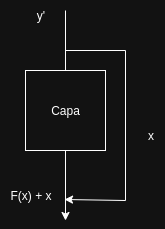
\includegraphics[width=0.5\linewidth]{img/ResNet.png}
    \caption{Ejemplo gráfico conexión residual}
    \label{fig:placeholder13}
\end{figure}

Esto se entiende mejor al calcular las derivadas parciales para actualizar los pesos en \textit{basckpropagation}. Como se observa en la siguiente expresión, el gradiente nunca se anula completamente gracias al término de identidad: 

\[
\frac{\partial \mathcal{E}}{\partial x}
= \frac{\partial \mathcal{E}}{\partial y}
    \frac{\partial y}{\partial x}
= \frac{\partial \mathcal{E}}{\partial y}
    \left( \frac{dF(x)}{dx} + 1 \right).
\]

De esta manera, incluso cuando $\frac{dF(x)}{dx}$ tiende a cero, el gradiente conserva la contribución de la identidad ($+1$). Así, la red es capaz de mantener un flujo estable de información hacia atrás, evitando que los gradientes mueran. Además, puede aprender a ignorar aquellas transformaciones que no sean beneficiosas en el entrenamiento, llevando sus pesos hacia cero y dejando pasar directamente la señal original $x$ \parencite{apxml_addnorm}. 

\subsubsection{Normalización (\textit{Layer Norm})}

Tras la conexión residual, se aplica una capa de normalización. A diferencia de otras capas de normalización, como la normalización por lotes (\textit{Batch Norm}), que normaliza los datos a lo largo del lote de entrenamiento, la normalización por capas (\textit{Layer Norm}) lo hace para cada muestra individual en sus características internas. Esto es especialmente importante en NLP, donde las secuencias de entrada pueden variar en longitud y contenido y no interesa que cada una se vea afectada por estadísticas de otra. Además, si se usase la normalización por lotes, se haría \textit{padding}, y los valores de relleno afectarían a las estadísticas de la normalización, especialmente en frases cortas. A continuación, se muestra un ejemplo que plasma claramente la diferencia entre ambas técnicas:

Dadas las siguiente secuencias: 

\[
\text{secuencia}_1 = [2,3], \quad \text{secuencia}_2 = [4,5]
\]

La normalización por lotes se aplica a lo largo del batch:
\[
\mu_1 = \frac{2 + 4}{2} = 3, 
\quad 
\sigma_1 = \sqrt{\frac{(2-3)^2 + (4-3)^2}{2}} = 1
\]

Mientras que la normalización por capa se aplica dentro de cada secuencia considerando todas sus características, así la posición 1:
\[
\mu_{\text{seq1}} = \frac{2 + 3}{2} = 2.5, 
\quad 
\sigma_{\text{seq1}} = \sqrt{\frac{(2-2.5)^2 + (3-2.5)^2}{2}} = 0.5
\]

\[
\mu_{\text{seq2}} = \frac{4 + 5}{2} = 4.5, 
\quad 
\sigma_{\text{seq2}} = \sqrt{\frac{(4-4.5)^2 + (5-4.5)^2}{2}} = 0.5
\]


Con ello, en base a estas dos operaciones, de media y varianza, se realzia la normalización de los valores de entrada en cada capa aplicando la siguiente expresión: 

\begin{equation}
    \hat{x}_i = \frac{x_i - \mu}{\sqrt{\sigma^2 + \epsilon}} \cdot \gamma + \beta
    \label{eq:normalization_sigma}
\end{equation}


En dicha expresión se observan dos parámetros entrenables, $\gamma$ y $\beta$, que permiten al modelo aprender la escala y el desplazamiento óptimos para cada característica. Sin estos parámetros, la normalización es demasiado restrictiva, pues los resultados se aplanan siempre a un mismo rango. El término $\epsilon$ es un valor pequeño añadido para evitar divisiones por cero y garantizar la estabilidad numérica.

Otra de las ventajas de normalizar es que mitiga el \textit{internal covariate shift} \parencite{sharma2024addnorm}. Durante el entrenamiento las distribuciones de las activaciones cambian, dado que los pesos cambian, lo que ralentiza la convergencia \parencite{apxml_addnorm}, haciendo el entrenamiento más inestable y el optimizador pierde tiempo corrigiendo desajustes. Gracias a la normalización, las variables se mantienen en una escala controlada.


\subsection{Feed Forward} \label{subsec:feedforward}
En términos generales se trata del proceso por el que la información pasa a través de una red, únicamente en sentido hacia delante, desde su entrada hasta su salida, pasando por todas las capas ocultas que hubiese. 

Se define como una capa o bloque que toma la salida de la capa de atención y la procesa a través de una red neuronal densa, esto es, totalmente conectada. Esta red consta de dos capas lineales con una función de activación no lineal entre ellas, que en el paper original es ReLU. La primera capa expande la dimensionalidad del embedding, mientras que la segunda la reduce de nuevo a su tamaño original. Esto permite al modelo aprender representaciones más complejas y captar interacciones no lineales, lo cual es un factor importante pues permite, por ejemplo, que el modelo entienda el contexto y significado de una palabra en función de donde aparece en la frase \parencite{kyeg_feedforward_demystified}.

Pese a que originalmente se usaban 2 capas lineales con ReLU, en la actualidad se ha demostrado una mejora significativa al aumentar el número de capas, obteniendo un entrenamiento más estable, pues se vió que el aprendizaje al inicio era mayor, y reduciendo el problema por la desaparición del gradiente. Además, se ha demostrado ampliamente que es un bloque fundamental, pues en varios experimentos, al eliminar esta capa, el rendimiento del modelo disminuye drásticamente \parencite{gerber2025ffn}.


\subsection{Linear y softmax}
Las últimas capas del modelo son una capa lineal y softmax. A través de la primera se obtienen los denominados \textit{logits}, que son puntuaciones sin normalizar sobre que tan probable es cada token para el modelo. La función de esta capa es transformar los embeddings de alta dimensión en una representación que pueda ser interpretada como una distribución de probabilidad sobre el vocabulario.

A través de \textit{softmax}, se transforman estas puntuaciones en una distribución de probabilidad, donde cada valor representa la probabilidad de que un token específico sea el siguiente en la secuencia generada. 

%--- FIN DEL CAPÍTULO 3

\clearemptydoublepage

%--- CAPÍTULO 4 DEL TFM
\chapter{Resultados}
\section{Preparación del entorno}
El proyecto se implementa íntegramente en Python 3.12. 
El primer punto es montar un entorno virtual donde se instalarán las librerías necesarias.

\begin{lstlisting}[language=bash]
python3 -m venv .venv
source .venv/bin/activate
\end{lstlisting}
El segundo punto consiste en instalar \texttt{CUDA} y \texttt{Pytorch} y verificar que la GPU es detectada
\begin{lstlisting}[language=bash]
# Verificar CUDA, en mi caso tengo la version 12.9.
nvidia-smi

#Instalar torch para esa version de CUDA
pip install --pre torch torchvision torchaudio --index-url https://download.pytorch.org/whl/nightly/cu129
\end{lstlisting}

\begin{lstlisting}[language=Python]
import torch
print(torch.cuda.is_available())
print(torch.version.cuda)
print(torch.cuda.device_count())
\end{lstlisting}
En este caso, la GPU utilizada es: NVIDIA GeForce RTX 4090 Laptop GPU con memoria total (MB): 15943

\section{Análisis de los dataset}
\subsection{Tiny Shakespeare}
Se trata de un dataset creado por Andrej Karpathy compuesto por 40.000 líneas con las obras de Shakespeare. El dataset está disponible en HuggingFace \parencite{huggingface_tinyshakespeare}.

\begin{lstlisting}[language=bash]
wget https://raw.githubusercontent.com/karpathy/char-rnn/master/data/tinyshakespeare/input.txt -O tinyshakespeare.txt
\end{lstlisting}
\begin{figure}[h]
    \centering
    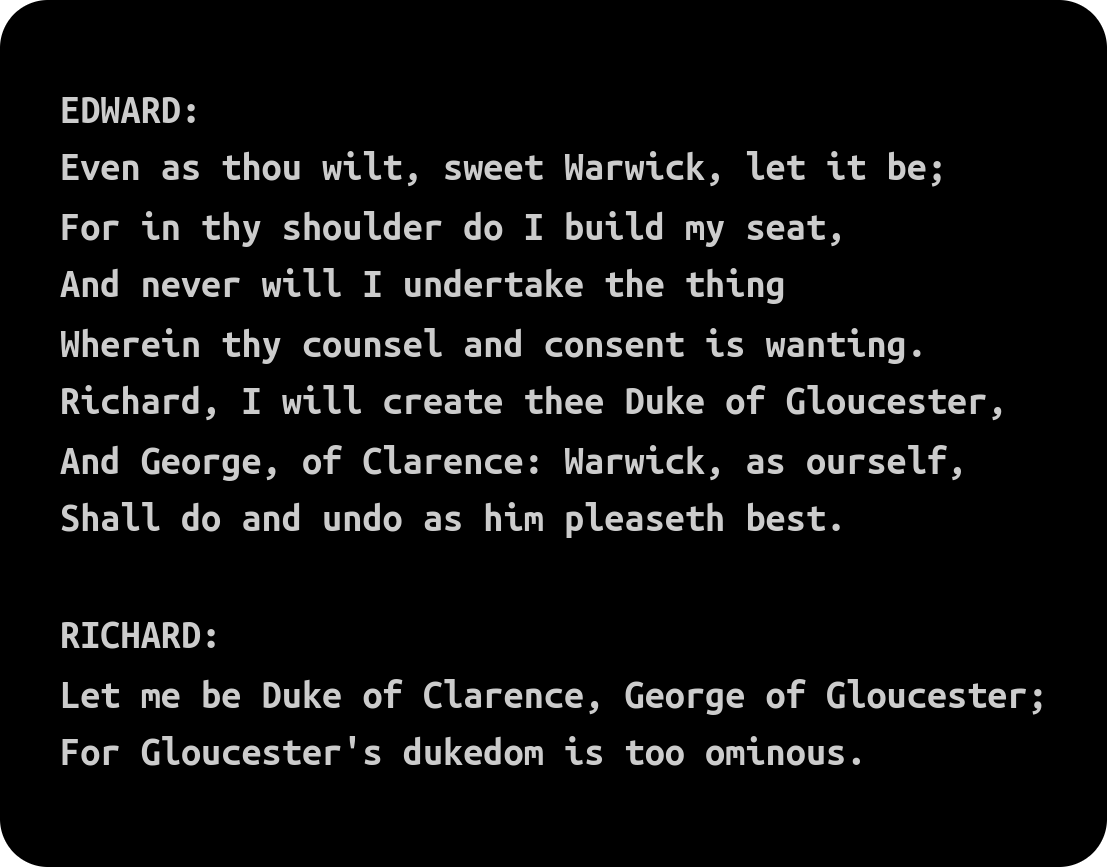
\includegraphics[width=0.5\linewidth]{img/tiny_shakespeare.png}
    \caption{Fragmento del dataset Tiny Shakespeare}
    \label{fig:placeholder1}
\end{figure}
\subsection{WikiText2}
Este dataset se puede descargar de Salesforce en Huggingface y consta de más de 2 millones de tokens de datos, divididos en 4358 ejemplos para test, 36718 para entrenamiento y 3760 para validación. Este contiene una colección de textos seleccionados de Wikipedia \parencite{huggingface_wikitext} \parencite{autonlp2020linkedwikitext}

\begin{lstlisting}[language=Python]
wikitext2 = load_dataset("Salesforce/wikitext", "wikitext-2-raw-v1")
\end{lstlisting}

\section{Limpieza y tokenización}
Para que el modelo sea capaz de encontrar patrones y llegar a "comprender" un texto, es necesario estructurarlo previamente. En sí, el proceso de estructuración consiste en aplicar una serie de reglas al texto para normalizarlo, limpiarlo y extraer los llamados "tokens". Un token se puede entender como un fragmento de un texto; puede ser, por ejemplo, un carácter, una palabra o una subpalabra. Estos tokens se transforman a un valor numérico, con lo que ya se tendría una representación numérica del texto, pero para que el modelo lo comprenda, cada token se representa como un vector o tensor, son los llamados embeddings, que capturan el contexto de las palabras y otra información importante. \parencite{lmpo2020bpe}


En lo referido a la limpieza del texto existen diversas técnicas, como limpiar etiquetas HTML, caracteres especiales, \textbf{stop words}, duplicados, convertir a minúsculas, solucionar problemas de encoding, lematización o corrección de palabras (librerías de Python como SpellChecker permiten realizar esta tarea) \parencite{shabbir2021cleaning}. En este proyecto, dado que los datasets empleados ya están correctamente procesados y se va a utilizar un tokenizador Byte-Pair encoding (BPE) a través de SentencePiece, no es necesario un pre-procesamiento demasiado exhaustivo, se limita a corrección de posibles problemas de codificación utilizando \textbf{ftfy}, espacios en blanco y normalización de comillas y guiones usando unicode.

\begin{figure}[h]
    \centering
    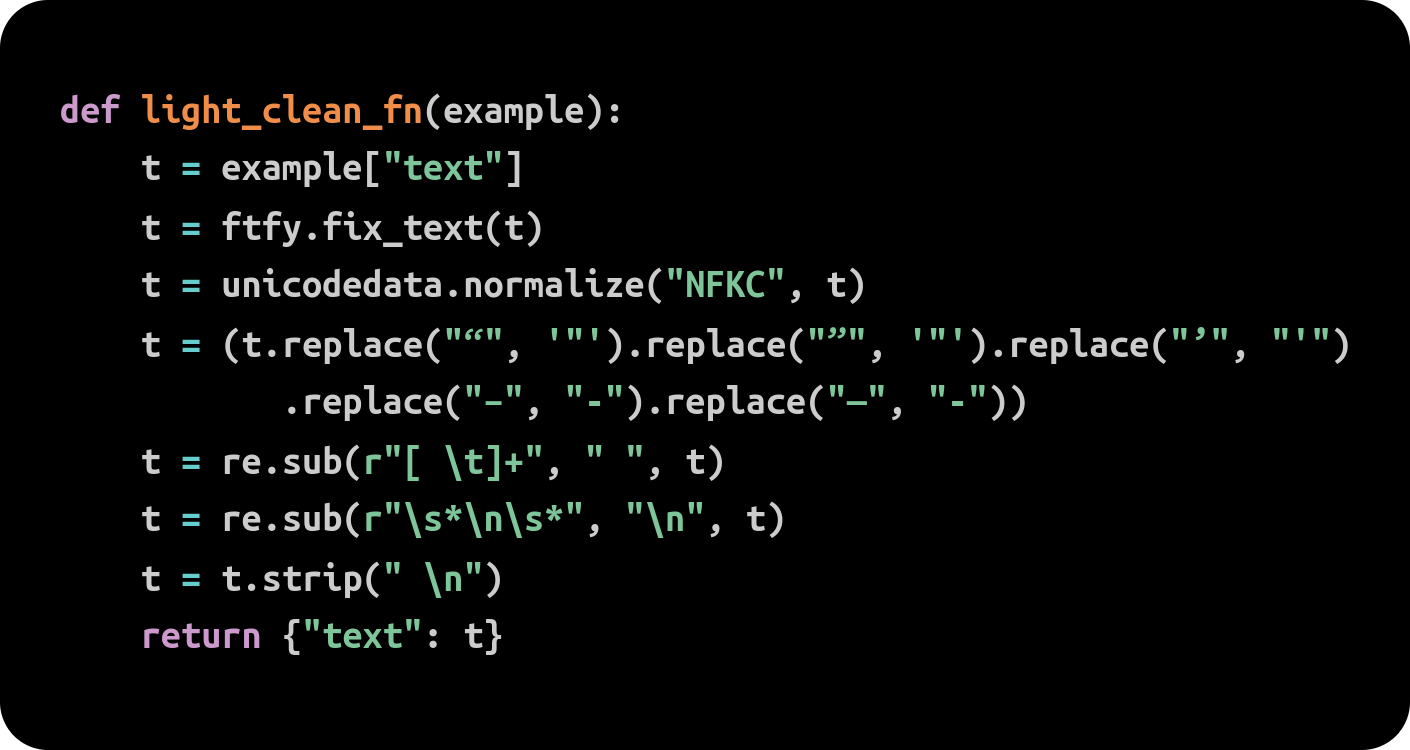
\includegraphics[width=0.5\linewidth]{img/preclean.png}
    \caption{Limpieza antes de tokenizar}
    \label{fig:placeholder2}
\end{figure}
Como se ha mencionado, existen distintas técnicas de tokenización. A nivel más simple está la tokenización en caracteres, en palabras y en subpalabras. La primera tiene la ventaja de disminuir la complejidad, sin embargo, el modelo está más limitado a la hora de aprender representaciones significativas. Puede ser útil para idiomas como el chino, donde la morfología es compleja y no existen los espacios. La segunda es la tokenización por espacio y puntuación, es decir, la frase \textit{"Mi perro come mucho."} no se descompone en los tokens: \textit{"Mi", "perro", "come", "mucho."}, que es a lo que equivaldría hacer un split por espacios, sino que se tokenizaría como: \textit{"Mi", "perro", "come", "mucho", "."}. El problema de este método es la complejidad en memoria y tiempo, pues genera un vocabulario muy grande y con ellos una matriz de embeddings también demasiado grande. A esto hay que sumar que aparece el problema de palabras no vistas o \textit{UNK}. 
Estos problemas se resuelven con la tokenización de subpalabras. Este método se basa en la idea de que las palabras que se usan con frecuencia no deberían dividirse, mientras que las más raras sí, manteniendo así palabras más frecuentes. Por ejemplo, en un texto en inglés, la palabra \textit{"annoyingly"} no es una palabra común, mientras que las subpalabras \textit{"annoying"} y \textit{"ly"} sí. Permite, con ello, ver más vocabulario, sin perder significado de las palabras menos frecuentes \parencite{lmpo2020bpe}

En este proyecto, dado que son textos en inglés y las limitaciones técnicas que existen, se ha decidido utilizar un tokenizador de subpalabras. Entre estos, destacan dos: BPE y WordPiece \parencite{huggingface_tokenizer_summary}. Ambos funcionan de forma similar, la principal diferencia radica en cómo realizan las "uniones" a partir del vocabulario base. BPE lo que hace es primeramente una pre-tokenización de los datos de entrenamiento por espacios o basada en reglas (por ejemplo, \textbf{Moses}). Con ello, obtiene un conjunto de palabras únicas y su frecuencia. Tras ello, crea un vocabulario base con los distintos símbolos que aparecen en las palabras únicas. La idea ahora es aprender reglas de unión para crear nuevos símbolos a partir de otros dos en base a la frecuencia. El proceso se repite hasta alcanzar el tamaño deseado, que se configura como hiperparámetro. \textbf{En GPT el tamaño es de 40478 tokens.} Para evitar un vocabulario base muy extenso si se quiere tener todos los caracteres con el fin de evitar palabras o tokens no vistos, se pueden usar bytes, así se tiene un tamaño fijo de 256, utilizando reglas para los caracteres de puntuación que no se puedan representar. \\
\\
\textbf{METER EJEMPLO}\\

WordPiece, en lugar de escoger simplemente los pares de símbolos más frecuentes, utiliza probabilidades. En sí, para cada par de símbolos, calcula la probabilidad combinada entre la individual de cada uno. El par con el valor de $\text{score}(A,B)$ más alto es el que se añade al vocabulario, ya que indica que ambos símbolos aparecen juntos con más probabilidad de la esperada si fueran independientes.\\

Dado que los \textit{datasets} que utilizo no son muy grandes, voy a emplear BPE con SentencePiece \parencite{google_sentencepiece}. Además, este método ha sido utilizado en modelos como GPT \parencite{reddit2021tokenizers}. 

SentencePiece es un framework de tokenización y detokenización desarrollado por Google que facilita la implementación de BPE. Entre sus características principales destaca el hecho de que no depende del idioma, ya que trabaja directamente con caracteres crudos, permite entrenar sin preprocesamiento previo y sin precisar librerías externas como NLTK o SpaCy, y trata los espacios en blanco como caracteres independientes, lo que resuelve problemas en lenguas sin segmentación explícita como el chino. El resultado es un modelo portable y eficiente. 

Asimismo, SentencePiece incluye mecanismos avanzados que mejoran la robustez de los modelos: 
\begin{itemize}
    \item \textbf{Byte fallback}, hace que si aparece cualquier caracter desconocido no genere un \textit{"UNK"}, sino que lo descompone en bytes.
    \item \textbf{BPE-dropout}, que introduce aleatoriedad en el proceso de segmentación durante el entrenamiento para mejorar la generalización, en sí lo que hace es omitir uniones aleatoriamente durante la tokenización.
    \item \textbf{Regularización por subpalabras}, que permite generar múltiples segmentaciones posibles de una misma secuencia, actuando como técnica de \textit{data augmentation}.
\end{itemize}


\[
\text{puntuación}(A,B) = \frac{P(AB)}{P(A) \cdot P(B)}
\]

donde:
\begin{itemize}
    \item $P(AB)$ es la probabilidad estimada de que aparezca el token combinado $AB$
    \item $P(A)$ y $P(B)$ son las probabilidades de cada símbolo por separado.
\end{itemize}
\text{\#\#\#\#\#\#\#\#\#\#\#\#\#\#\#\#\#\#\#\#\#\#\#\#\#\#\#\#\#\#\#\#\#}

\subsection{Implementación del tokenizador BPE}
El primer paso es entrenar el tokenizador, de forma que aprenda el vocabulario y a dividir en subpalabras. Se establece el tipo de modelo, "bpe" en este caso, el tamaño del vocabulario final, la porción de caracteres del corpus que debe cubrir el modelo (1 para cubrir todos) y el número de hilos de CPU a usar durante el entrenamiento. Además, se utiliza el parámetro \textit{byte\_fallback} para controlar los caracteres desconocidos, tal y como se ha explicado previamente.Se aplica una normalización NFKC (descompone los caracteres en formas básicas y los recompone siguiendo una forma estándar) antes de entrenar donde se estandarizan caracteres y eliminan espacios innecesarios o múltiples. Esto es algo que conviene usar con lenguajes como el japonés que utilizan caracteres desnormalizados o textos sucios y desnormalizados; sin embargo, en este caso, los datasets empleados ya están listos para usarse y se podría evitar. Por último, se asignan los IDs especiales:

 \begin{itemize}
     \item pad: token de padding para rellenar secuencias de distinta longitud.
     \item unk: Tokens desconocidos, pese a estar controlados con el parámetro mencionado.
     \item bos: Token de inicio de secuencia, para dar consistencia.
     \item eos: Token de fin de secuencia. Permite al modelo a aprender a parar.
 \end{itemize}
\begin{figure}[h]
    \centering
    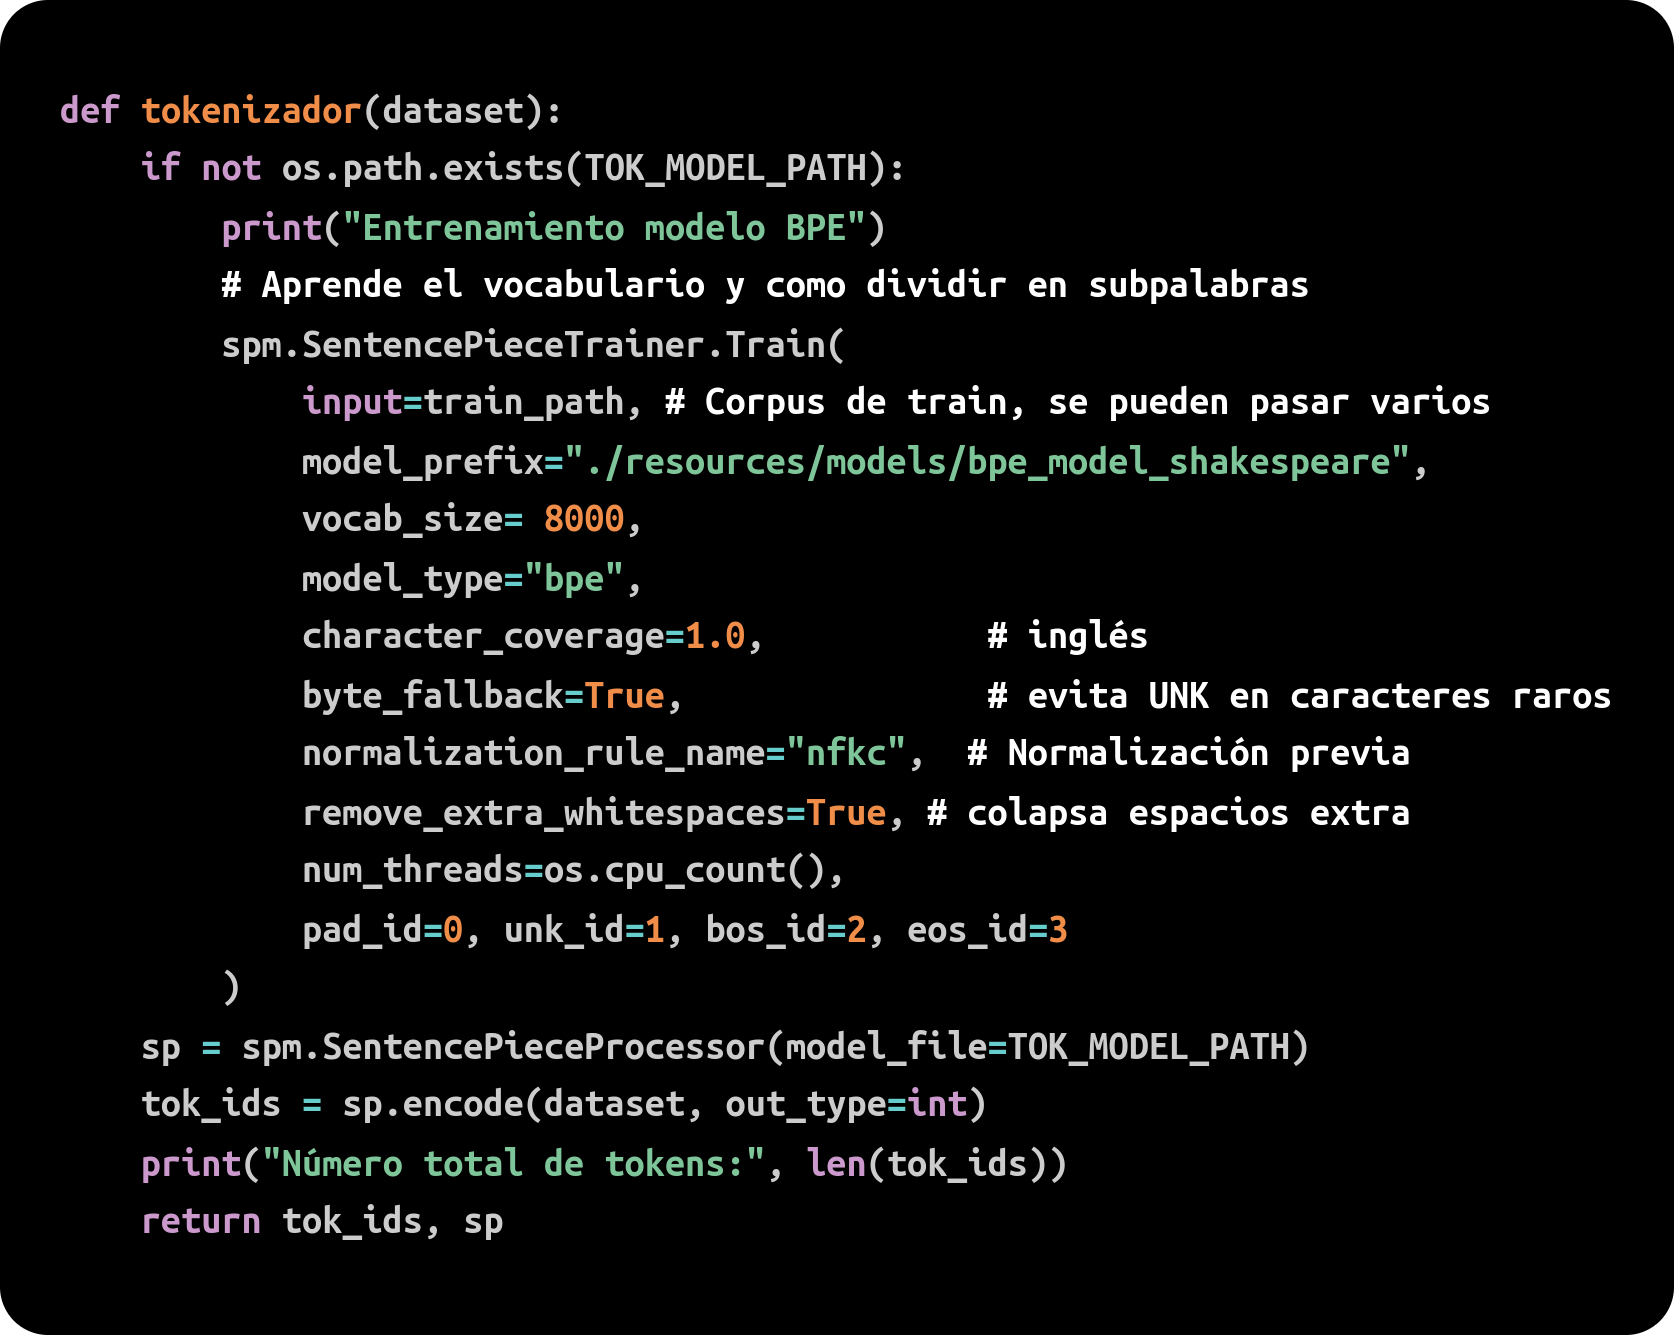
\includegraphics[width=0.5\linewidth]{img/sentence_trainer.png}
    \caption{Enter Caption}
    \label{fig:placeholder3}
\end{figure}
 
Una vez entrenado el tokenizador, se procede a tokenizar los conjuntos de datos (\textit{train}, \textit{validation} y \textit{test}) utilizando dicho modelo. Para ello, se definen las siguientes funciones:

\begin{itemize}
    \item \textbf{\texttt{sp\_encode\_batch\_train}}: utilizada para tokenizar los datos de entrenamiento. Esta función habilita el muestreo probabilístico de segmentaciones (\textit{subword regularization}) mediante los parámetros \texttt{enable\_sampling=True}, \texttt{nbest\_size=-1} y \texttt{alpha=0.1}. Esta técnica introduce pequeñas variaciones en las secuencias tokenizadas para un mismo texto, lo que actúa como regularización durante el entrenamiento del modelo de lenguaje.
\begin{figure}[h]
    \centering
    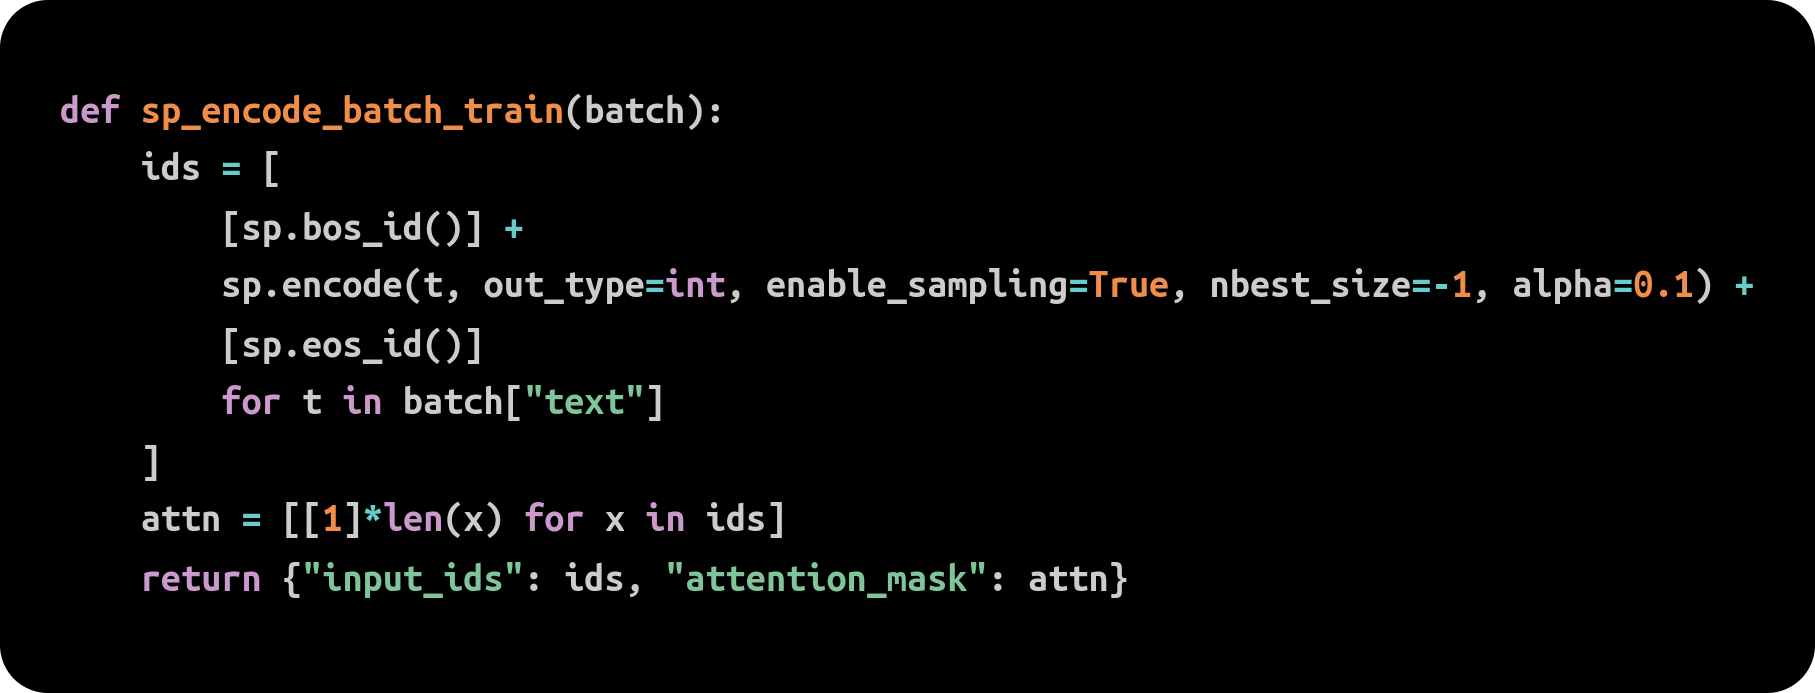
\includegraphics[width=0.5\linewidth]{img/train_tok.png}
    \caption{Enter Caption}
    \label{fig:placeholder4}
\end{figure}
    \item \textbf{\texttt{sp\_encode\_batch\_eval}}: usada para tokenizar los conjuntos de validación y prueba. Aquí se desactiva el muestreo para que la tokenización sea determinista y reproducible.

    \begin{figure}[h]
        \centering
        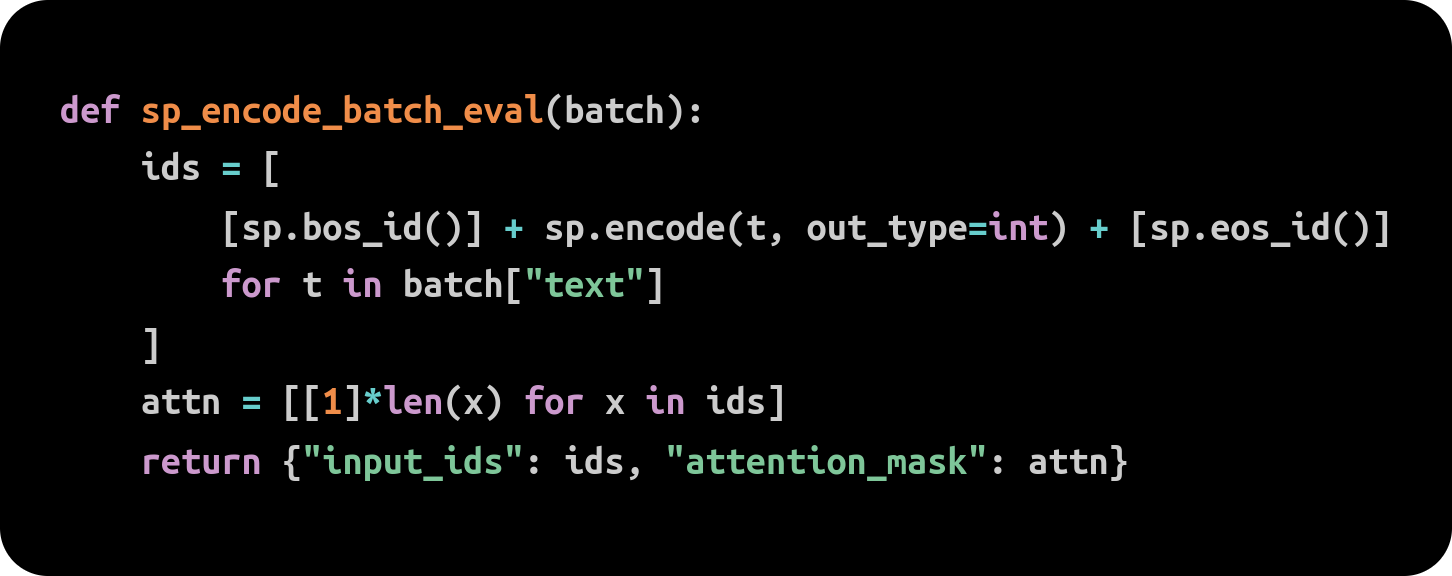
\includegraphics[width=0.5\linewidth]{img/test_tok.png}
        \caption{Enter Caption}
        \label{fig:placeholder5}
    \end{figure}
\end{itemize}

En ambos casos, a cada secuencia tokenizada se le añaden explícitamente los tokens especiales de inicio (\texttt{<bos>}) y fin (\texttt{<eos>}) de secuencia, cuyos IDs fueron definidos durante el entrenamiento del modelo SentencePiece. Además, se genera una máscara de atención (\texttt{attention\_mask}) compuesta inicialmente por unos, ya que en este punto todavía no se ha aplicado \textit{padding}.

\paragraph{Ejemplo:}

Considerando la frase:

\begin{quote}
\texttt{El perro ladra en el prado}
\end{quote}

La función \texttt{sp.encode(...)} devuelve una secuencia de IDs correspondiente a las subpalabras identificadas por SentencePiece. Por ejemplo:

\begin{center}
\texttt{[120, 457, 98, 14, 120, 892]}
\end{center}

donde los números representan los IDs de tokens correspondientes a subpalabras como:

\begin{quote}
\texttt{["\_El", "\_perro", "\_ladra", "\_en", "\_el", "\_prado"]}
\end{quote}

Si los IDs de los tokens especiales son \texttt{<bos> = 1} y \texttt{<eos> = 2}, entonces la secuencia final de entrada (\texttt{input\_ids}) será:

\begin{center}
\texttt{[1, 120, 457, 98, 14, 120, 892, 2]}
\end{center}

La correspondiente máscara de atención generada será:

\begin{center}
\texttt{[1, 1, 1, 1, 1, 1, 1, 1]}
\end{center}

\paragraph{Agrupación en lotes y padding:}

Supongamos ahora que otra frase más corta, como:

\begin{quote}
\texttt{El perro ladra}
\end{quote}

es tokenizada como:

\begin{center}
\texttt{[1, 120, 457, 98, 2]}
\end{center}

con la máscara:

\begin{center}
\texttt{[1, 1, 1, 1, 1]}
\end{center}

Al agrupar ambas secuencias en un mismo lote (\textit{batch}), se aplica \textit{padding} con un token especial (por ejemplo, \texttt{<pad> = 3}) para igualar su longitud. Las secuencias quedarían así:

\begin{itemize}
    \item \texttt{input\_ids}: \texttt{[1, 120, 457, 98, 14, 120, 892, 2]} \\
    \texttt{[1, 120, 457, 98, 2, 3, 3, 3]}
    \item \texttt{attention\_mask}: \texttt{[1, 1, 1, 1, 1, 1, 1, 1]} \\
    \texttt{[1, 1, 1, 1, 1, 0, 0, 0]}
\end{itemize}

Esta máscara de atención es utilizada por el modelo Transformer para ignorar las posiciones de padding durante el cálculo de las atenciones.

\text{\#\#\#\#\#\#\#\#\#\#\#\#\#\#\#\#\#\#\#\#\#\#\#\#\#\#\#\#\#\#\#\#\#}

\section{Embeddings y Positional Encodding}
Cualquier modelo basado en redes neuronales requiere que sus entradas sean valores numéricos, no arbitrarios, para poder trabajar con el lenguaje humano. Es cierto que los tokens del texto ya se han convertido a índices enteros usando técnicas de tokenización; no obstante, estos valores no son suficientes para que el modelo sea capaz de inferir relaciones semánticas entre las palabras y llegar a entender su significado.

Hay técnicas como  \textit{One-Hot Encoding} que representan cada palabra como un vector binario en el que solo una posición es 1 y el resto son ceros. Esto presenta varias desventajas: genera vectores de alta dimensionalidad, dispersos y no capturan ningún tipo de información sobre el significado, el contexto o la similitud entre palabras.

Es por ello que se utilizan ampliamente los \textit{embeddings}. En sí, se trata de vectores densos, de números reales, capaces de capturar el significado de las palabras, sus relaciones semánticas y su contexto dentro del lenguaje. Los embeddings se obtienen mediante entrenamiento, de manera que palabras con contextos similares tienden a tener vectores cercanos entre sí en el espacio vectorial \parencite{geeksforgeeks_embedding}.

\begin{figure}[h]
    \centering
    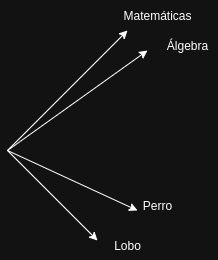
\includegraphics[width=0.5\linewidth]{img/ejemplo_embedding.png}
    \caption{Ejemplo similitud vectorial embeddings}
    \label{fig:placeholder6}
\end{figure}

Internamente, un embedding se representa como una matriz de pesos $E \in \mathbb{R}^{V \times d}$, donde $V$ es el tamaño del vocabulario y $d$ la dimensión del embedding. Cada fila de $E$ contiene el vector asociado a un token. Durante el entrenamiento, solo se actualizan los vectores correspondientes a los tokens presentes en cada lote, lo que permite un aprendizaje eficiente.\\

Otra ventaja de estos vectores multidimensionales es la posibilidad de operar con ellos, así un ejemplo clásico a la hora de hablar de embeddings, demuestra cómo capturan el contexto: 
\[
\text{vec}(\text{``rey''}) - \text{vec}(\text{``hombre''}) + \text{vec}(\text{``mujer''}) \approx \text{vec}(\text{``reina''})
\]

En modelos avanzados como los Transformers, los embeddings se combinan con codificaciones posicionales para incorporar la información del orden de las palabras en la secuencia. Esta suma permite que el modelo tenga acceso tanto al significado individual de las palabras como a su posición relativa dentro de la frase. Así puede capturar diferencias según dónde aparezca la palabra, no es lo mismo "un banco de peces" que "dinero en el banco".\parencite{perez_embeddings}

Esta matriz contiene información semántica de las palabras, pero dado que este tipo de arquitecturas procesan las secuencias en paralelo,  falta información sobre la posición de dichas palabras. A continuación se presenta una solución a este problema, es lo que se conoce como Positional Encoding. 

\subsubsection{Implementación embeddings}
Para mapear los índices resultantes de la tokenización a una matriz de \textit{embeddings}, se implementará una capa de embedding utilizando \texttt{PyTorch}. Esta capa actúa como una tabla de búsqueda que asocia cada índice con un vector de características. Internamente, se trata de una matriz de pesos que se optimiza durante el proceso de entrenamiento del modelo.

\begin{figure}[h]
    \centering
    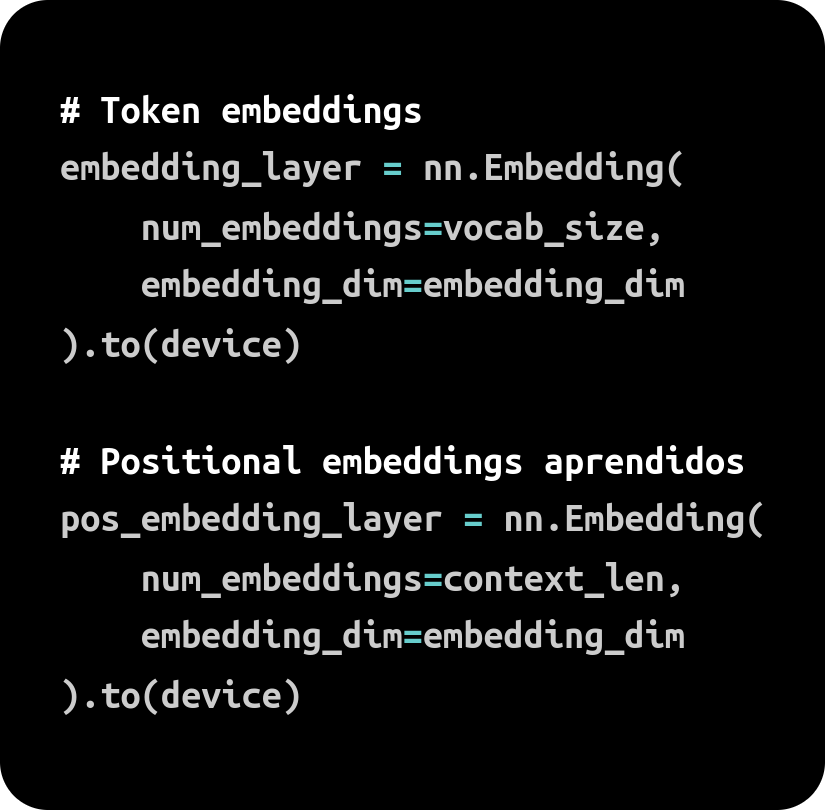
\includegraphics[width=0.5\linewidth]{img/embeddings1.png}
    \caption{Embeddings}
    \label{fig:placeholder17}
\end{figure}

Cabe destacar que inicialmente la matriz de embeddings se encuentra aleatorizada. A medida que se entrena el modelo, estos vectores se ajustan mediante retropropagación, lo que reduce la función de pérdida y permite que los embeddings capturen mejor la semántica, el contexto y otras relaciones relevantes entre los tokens. El resultado final es un tensor en el que cada fila representa un vector denso asociado a un token del vocabulario, adaptado a la tarea específica \parencite{bao2022embedding}. Se ha decidido inicializar los pesos siguiendo una inicialización Normal (ver sección \ref{sec:normal} del Anexo), lo que permite que inicialmente sean valores cercanos a 0, evitando que algunos tokens tengan valores demasiado grandes. 

\begin{figure}[h]
    \centering
    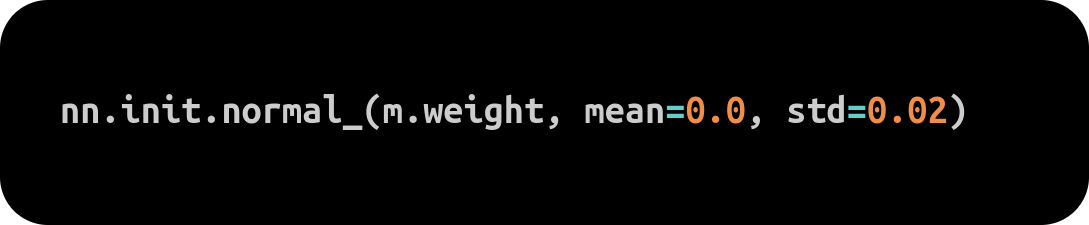
\includegraphics[width=0.5\linewidth]{img/normal_init.png}
    \caption{Inicialización Normal}
    \label{fig:placeholder18}
\end{figure}


\section{Mecanismos de atención}
La base de la arquitectura Transformer es la atención. A través de la atención, cada palabra mira simultáneamente al resto y calcula una métrica de relevancia a través de la cual, se determina que fracción de la información real es relavante para cada token y cpor tanto, para el modelo. 

Como se ha mencionado previamente, se basa en 3 matrices entrenables, inicializadas originalmente con valores aleatorios, y una operación, softmax, que calcula una distribución de probabilidad para cada token (ver \cref{subsec:multihead}).


\subsection{Implementación mecanismo de atención}
Usando \texttt{PyTorch} es posible trabajar de forma sencilla con tensores y replicar toda la lógica operacional. En primer lugar, se implementa un mecanismo de atención aplicando una máscara causal, a continuación se desarrolla la lógica de múltiples cabezas para capturar distintas relaciones entre los tokens.

El primer punto es crear las matrices de pesos \[W_Q, W_K, W_V\]. Aquí, \texttt{PyTorch} ofrece el módulo \texttt{nn.Linear}, que lo que hace es aplicar una transformación lineal (\[y = xW^T + b\]) a los datos de entrada \parencite{kanaries_nnlinear}, incializando aleatoriamente una matriz de pesos y un vector de sesgos, el cual, en este caso, no se va a inicializar pues no interesa que los vectores se desplacen en el espacio. Este módulo, toma dos parámetros: \textit{in\_features} y \textit{out\_features}, y la matriz resultante tiene un tamaño: \[\textit{in\_features} * \textit{out\_features}\]


De este modo, a partir de la misma entrada $x \in \mathbb{R}^{B \times T \times d_{model}}$ 
(secuencia de embeddings), se obtienen tres vistas distintas que serán usadas 
posteriormente en el cálculo de la atención.

\begin{figure}[h]
    \centering
    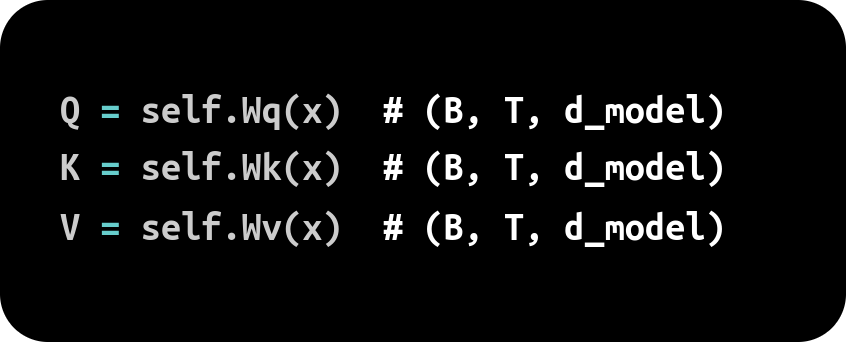
\includegraphics[width=0.5\linewidth]{img/Q_K_V.png}
    \caption{Proyección matrices Q, K, V}
    \label{fig:Proyeccion8}
\end{figure}

Los siguientes pasos son crear la métrica de atención, normalizar con softmax y aplicar los \textit{scores} a la información real. Con PytTorch es muy sencillo de realizar a través de las funciones \textit{matmul}, que permite multiplicar tensores, y \textbf{softmax}. 

\begin{figure}[h]
    \centering
    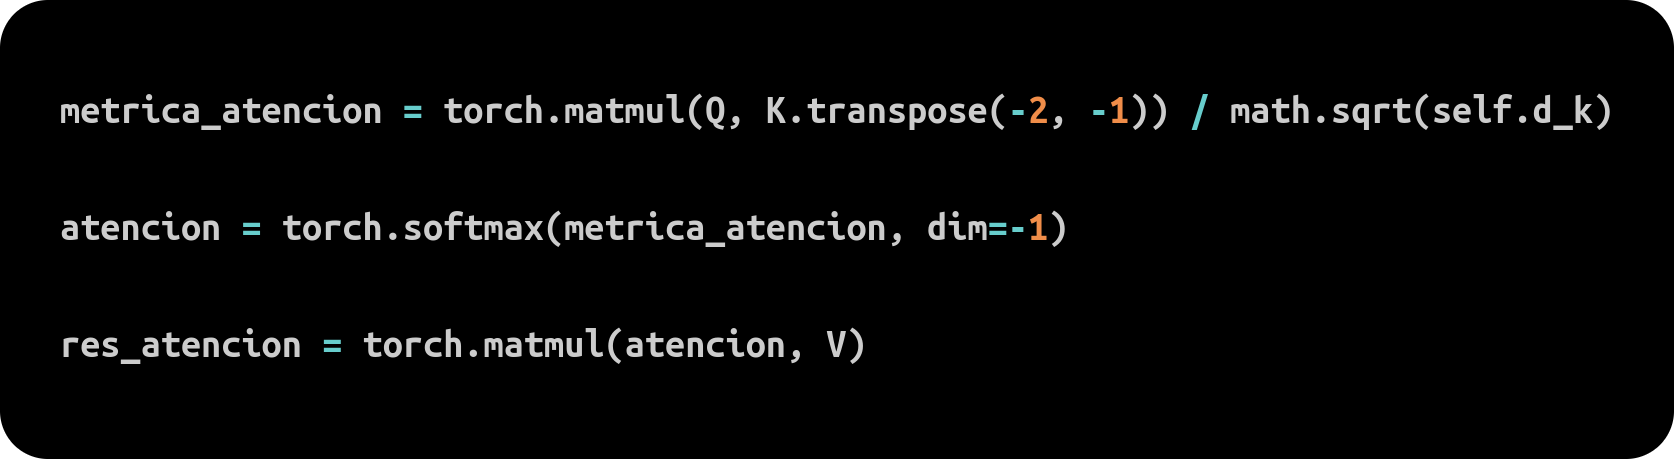
\includegraphics[width=0.5\linewidth]{img/atencion.png}
    \caption{Implementación Self Attention}
    \label{fig:placeholder9}
\end{figure}

Por último, queda aplicar la máscara de atención. Dado que el modelo implementado es de carácter autorregresivo y emplea ventanas de tamaño fijo sin añadir \textit{padding}, únicamente es necesaria la \textbf{máscara causal}. Su implementación resulta sencilla: se construye una matriz triangular superior de unos, cuyos valores se reemplazan por $-\infty$. Esta operación se aplica antes de la normalización con la función \textit{softmax}, de manera que las posiciones enmascaradas reciben una probabilidad prácticamente nula y, en la práctica, el modelo las ignora.  

Por ejemplo, para una secuencia de longitud $T=4$, la matriz de \textit{metrica\_atencion} $S$ se transforma en:  

\[
metrica\_atencion' =
\begin{bmatrix}
s_{11} & -\infty & -\infty & -\infty \\
s_{21} & s_{22} & -\infty & -\infty \\
s_{31} & s_{32} & s_{33} & -\infty \\
s_{41} & s_{42} & s_{43} & s_{44}
\end{bmatrix}
\]

De este modo, cada token únicamente puede atenderse a sí mismo y a los anteriores, lo que garantiza la naturaleza autorregresiva del modelo.

\begin{figure}[h]
    \centering
    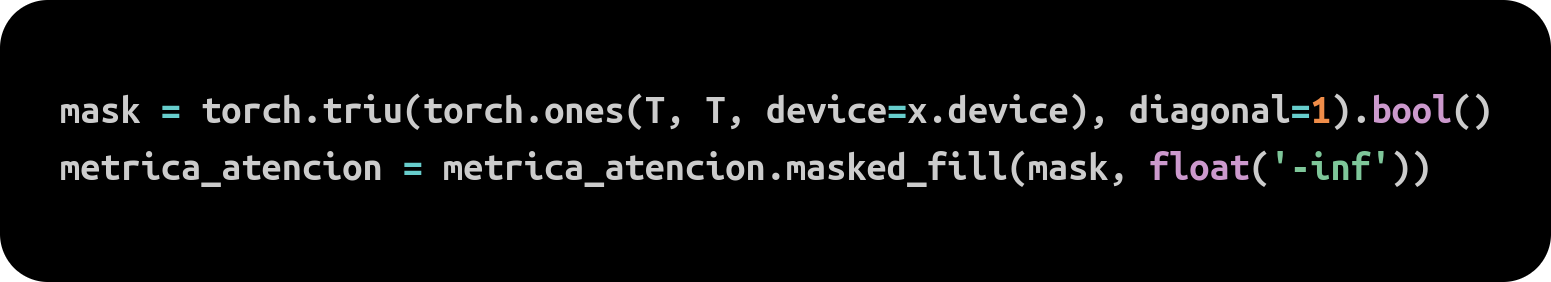
\includegraphics[width=0.5\linewidth]{img/masked.png}
    \caption{Implementación máscara causal}
    \label{fig:placeholder10}
\end{figure}

\subsection{Implementación de las múltiples cabezas de atención}
Para poder aplicar la atención múltiple las matrices originales Q, K, V se reorganizan en múltiples cabezas. Para ello, se emplea la función \texttt{view} de \texttt{PyTorch}, que permite reorganizar el tensor sin modificar sus datos en memoria. En este caso, se pasa de una estructura de tamaño $(B, T, d_{model})$ a otra de tamaño $(B, \textit{num\_heads}, T, d_k)$, donde $d_k = d_{model} / \textit{num\_heads}$ es la dimensión de cada cabeza. Posteriormente, se aplica una transposición para situar la dimensión de las cabezas en la segunda posición:

\begin{figure}[h]
    \centering
    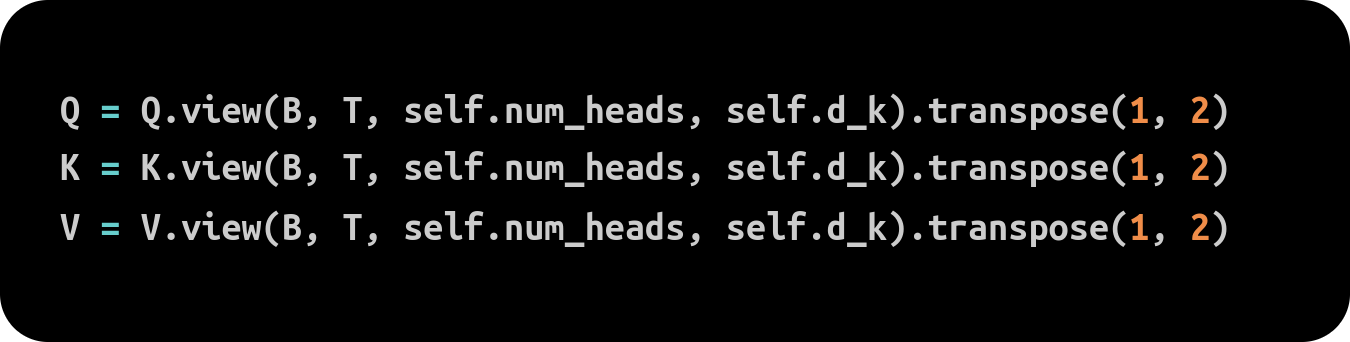
\includegraphics[width=0.5\linewidth]{img/heads.png}
    \caption{Implementación Multi-Head Attention}
    \label{fig:placeholder11}
\end{figure}

De este modo, cada cabeza de atención opera de manera independiente sobre un subespacio de dimensión $d_k$, calculando sus propios valores de similitud ($QK^T$) y generando una salida parcial. Finalmente, las salidas de todas las cabezas se concatenan de nuevo y se proyectan mediante una capa lineal adicional:

\begin{figure}[h]
    \centering
    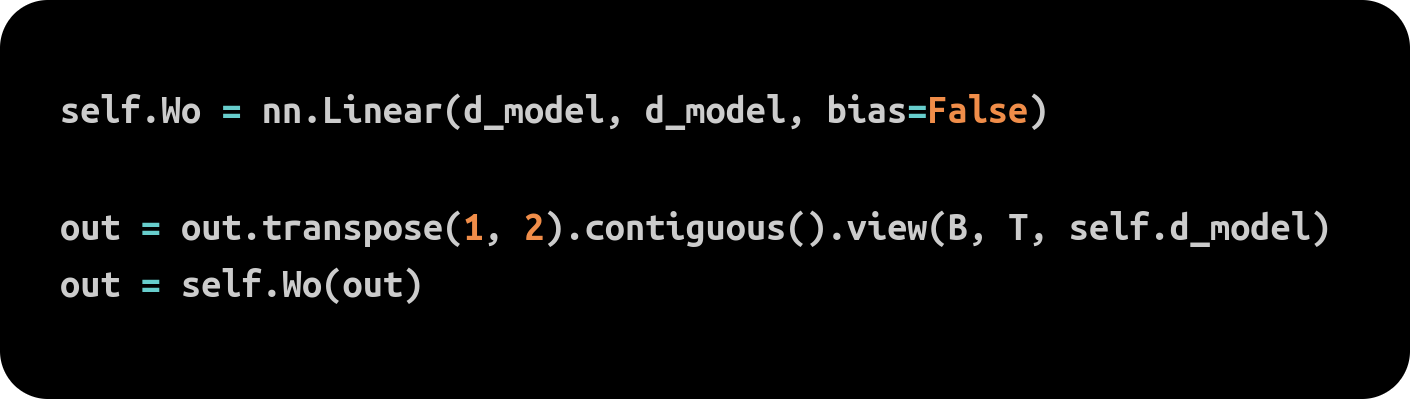
\includegraphics[width=0.5\linewidth]{img/heads2.png}
    \caption{Salida Multi-Head Attention}
    \label{fig:placeholder12}
\end{figure}

Por último, mencionar que la inicialización de los pesos se realiza mediante el método \textit{Xavier Uniform} (ver sección \ref{sec:xavier} del Anexo), que estabiliza el entrenamiento en capas profundas. 

\section{Normalización \texttt{(Add \& Norm)}}
Como se ha explicado en \ref{subsec:addnorm}, esta capa consta de dos elementos. Primero, una conexión residual que suma la entrada original a la salida del bloque de atención múltiple. En segundo lugar, una capa de normalización por capas que estabiliza y acelera el entrenamiento. En el siguiente esquema se visualiza mejor el flujo: 

\begin{figure}[h]
    \centering
    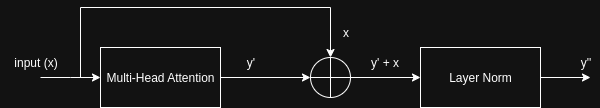
\includegraphics[width=0.5\linewidth]{img/esquema1.png}
    \caption{Flujo capa Add \& Norm}
    \label{fig:placeholder14}
\end{figure}

\subsection{Implementación Add \& Norm}

Como se puede ver en la imagen \ref{fig:placeholder26}, la conexión residual se realiza mediante una simple suma de tensores. La capa de normalización se ha implementado de cero, aunque \texttt{PyTorch} ofrece el módulo \texttt{nn.LayerNorm}, que realiza la misma función. En la implementación se calcula la media y la varianza por posición y devuelve el resultado de la expresión \eqref{eq:normalization_sigma}. 

Hay que señalar aquí el uso de \texttt{nn.Parameter} para los parámetros entrenables $\gamma$ y $\beta$. Se tratan como tensores especiales y se registran como parámetros entrenables del modelo, en concreto, se asocian a este módulo. 

\begin{figure}[h]
    \centering
    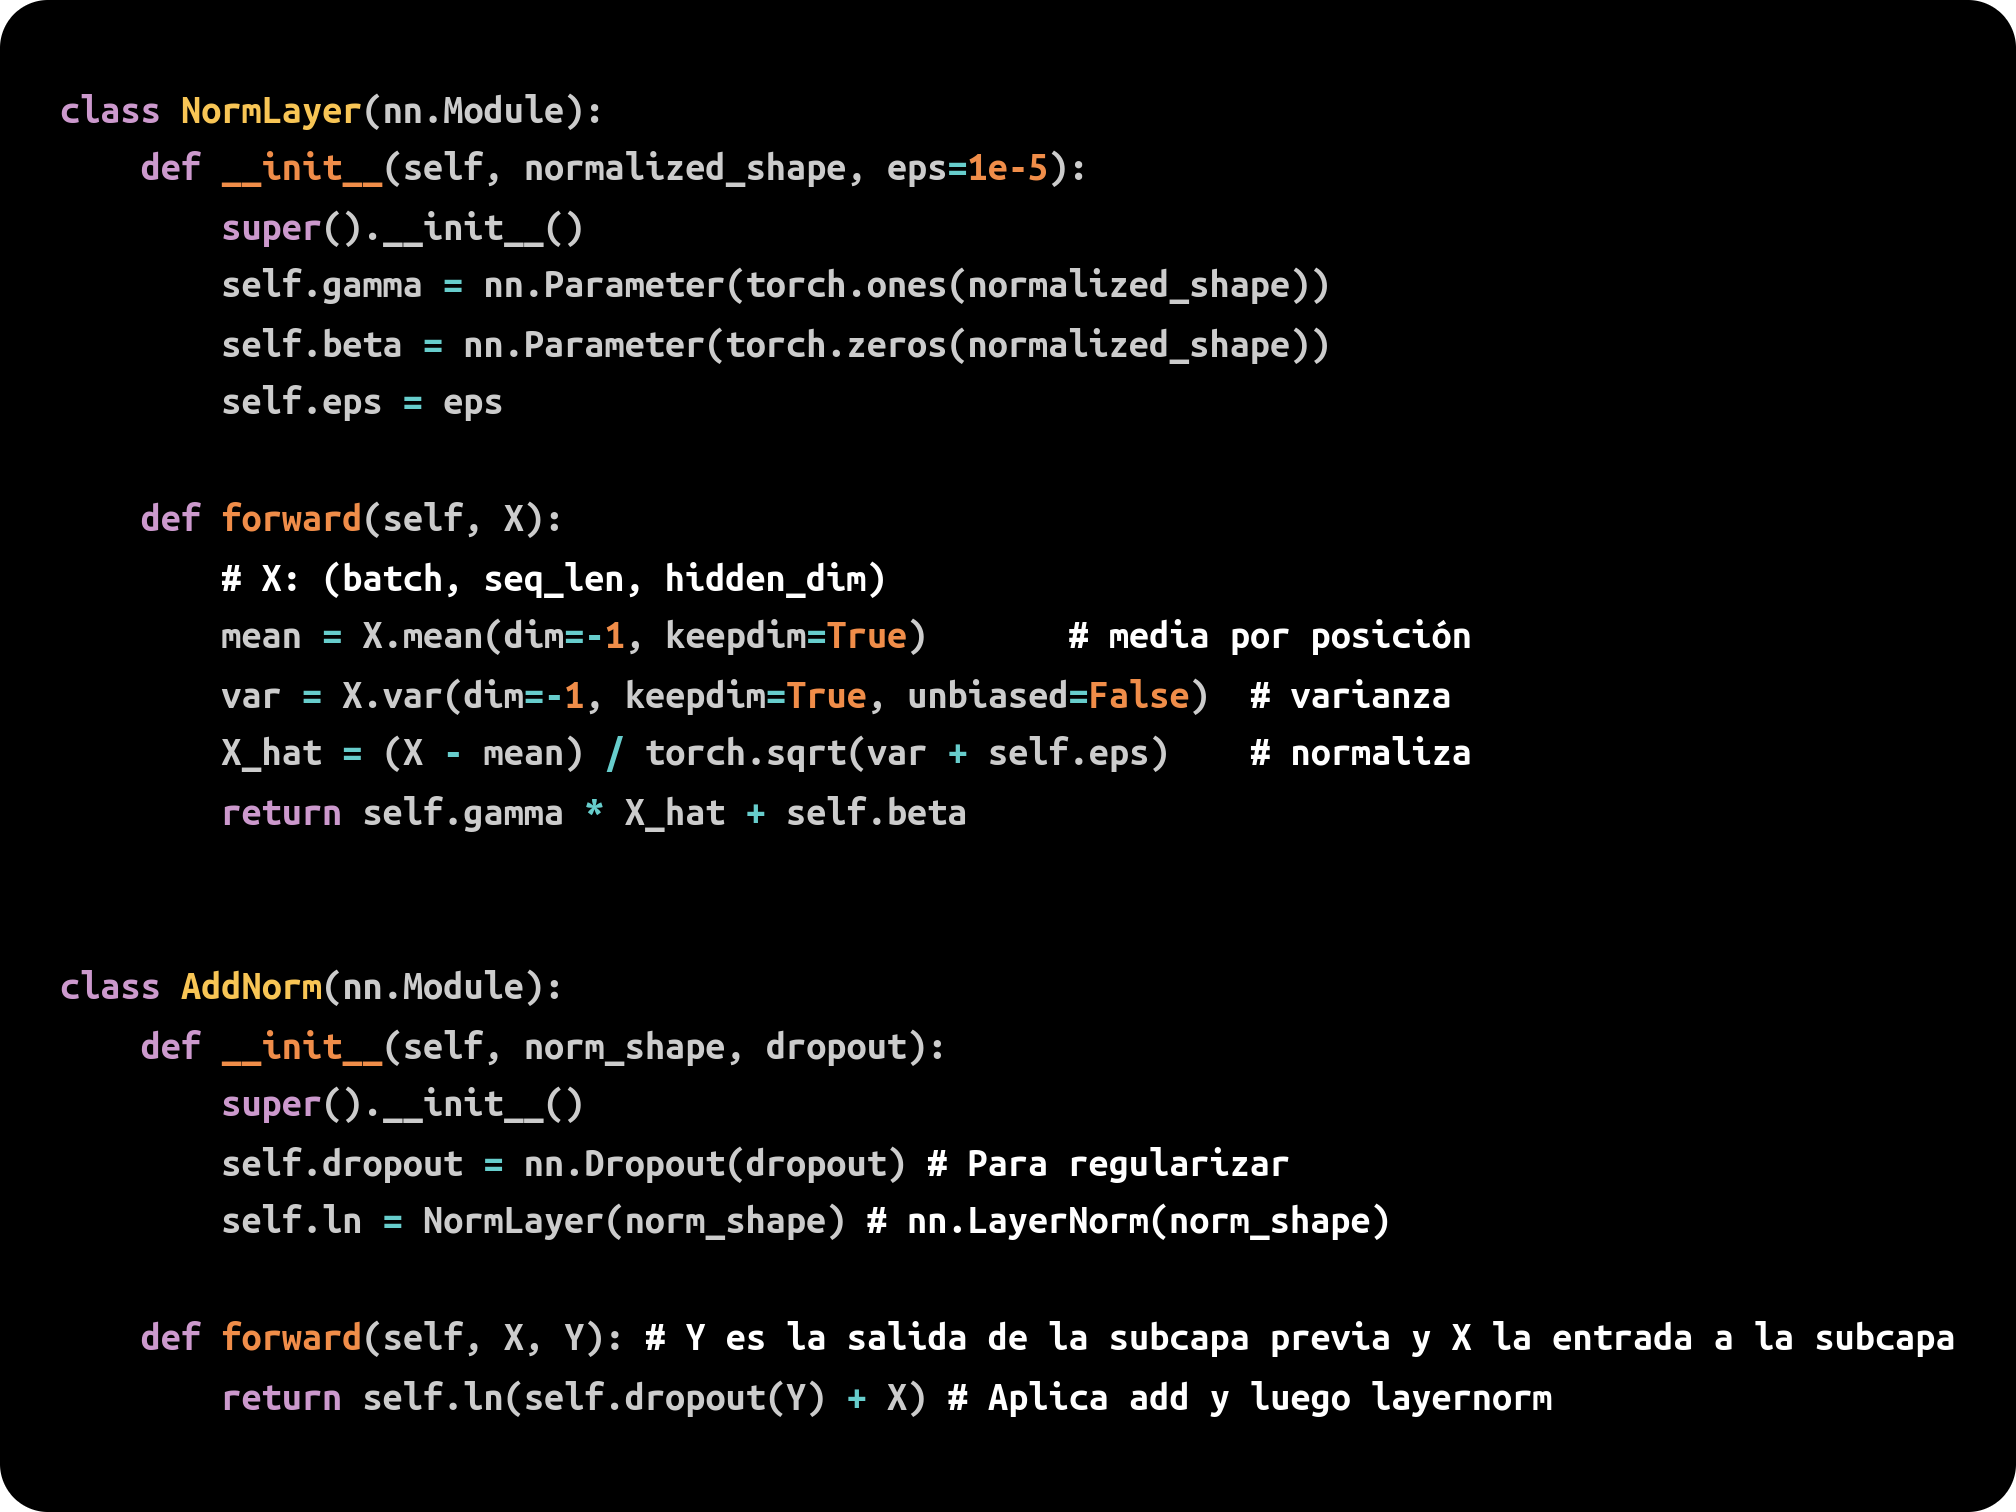
\includegraphics[width=0.5\linewidth]{img/add_norm.png}
    \caption{Implementación Add \& Norm}
    \label{fig:placeholder26}
\end{figure}

\section{Feed Forward} 
Tal y como se ha explicado en la sección \ref{subsec:feedforward}, el rendimiento del transformer es significativamente mejor al ampliar el número de capas lineales. Siguiendo las recomendaciones del paper \parencite{gerber2025ffn}, se ha decidido implementar 3 capas utilizando como función de activación \textit{GELU} (ver sección \ref{sec:gelu} del Anexo), que ha demostrado ser más efectiva que ReLU en este tipo de arquitecturas. La inicialización de los pesos se realiza mediante el método \textit{Xavier Uniform} al igual que en las capas de atención, para mantener la estabilidad del entrenamiento.

\begin{figure}[h]
    \centering
    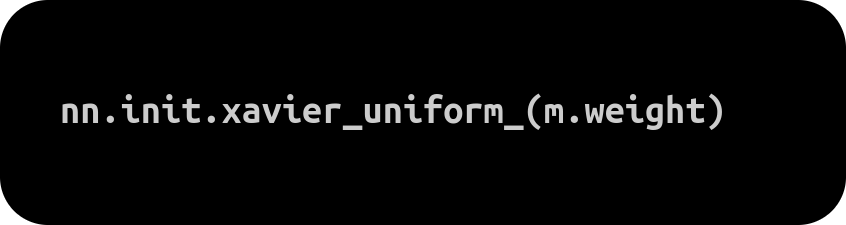
\includegraphics[width=0.5\linewidth]{img/xavier_init.png}
    \caption{Inicialización Xavier Uniform}
    \label{fig:placeholder15}
\end{figure}

La implementación es relativamente sencilla, se haría como si se tratara de un perceptrón multicapa \parencite{kyeg_feedforward_demystified}, donde se incluyen 3 capas lineales y dos funciones de activación GELU entre ellas. Además, se introduce \textit{dropout} para evitar sobreajuste, "apagando" aleatoriamente algunas neuronas durante el entrenamiento.

\begin{figure}[h]
    \centering
    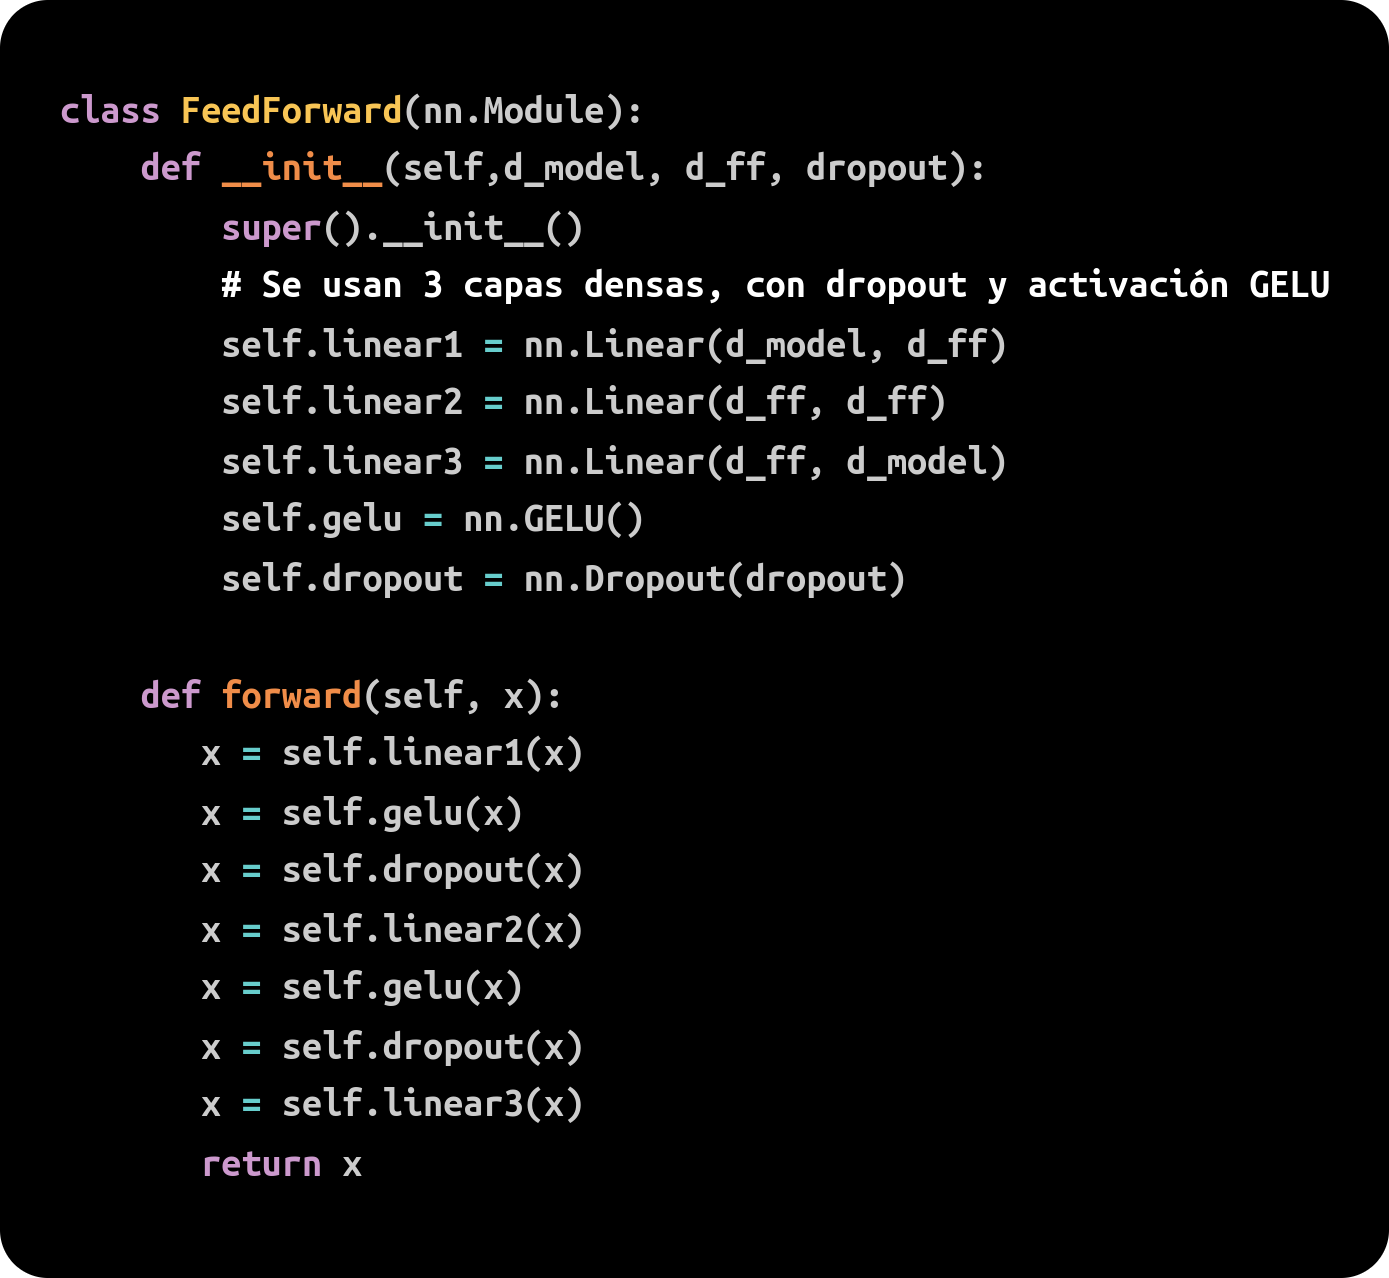
\includegraphics[width=0.5\linewidth]{img/ffnn.png}
    \caption{Capa FeedForward}
    \label{fig:placeholder16}
\end{figure}



\section{Entrenamiento}

Tras añadir la capa lineal de salida, tras el bloque \textit{transformer}, se finaliza las bases de la arquitectura Transformer \textit{decoder-only}. El siguiente paso es configurar los parámetros e implementar la infraestructura de entrenamiento del modelo. 

\begin{figure}[h]
    \centering
    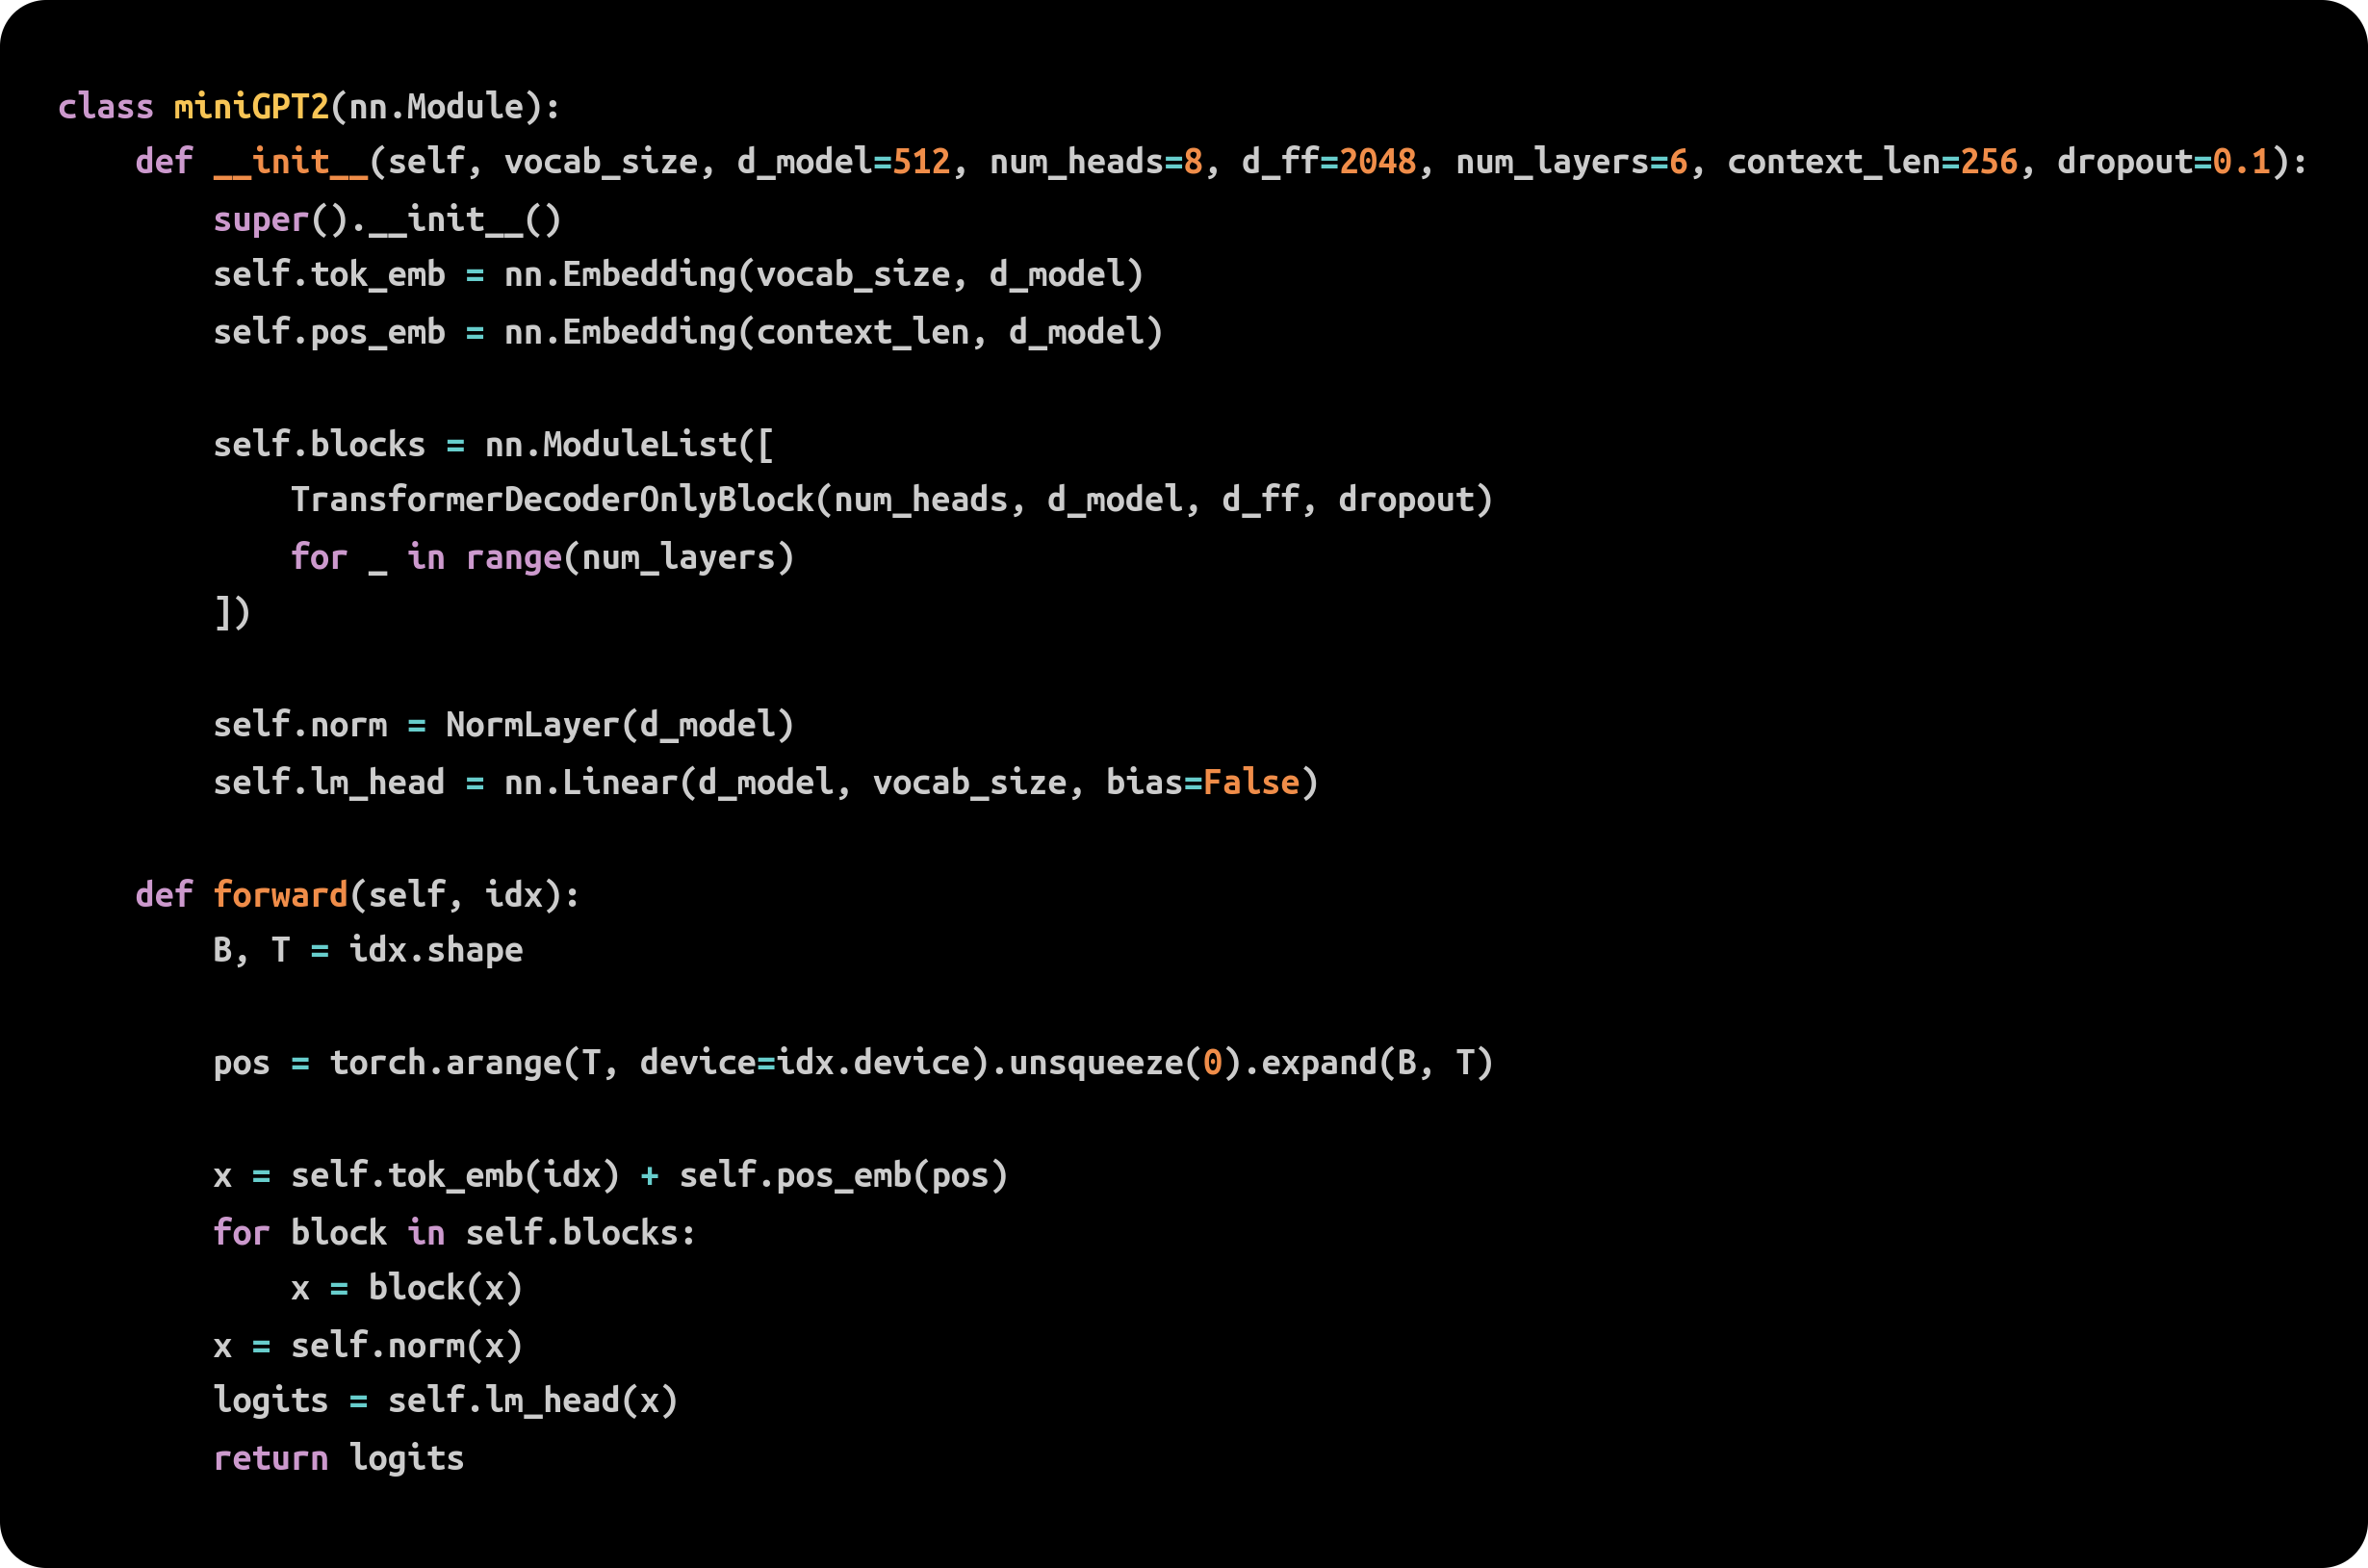
\includegraphics[width=0.5\linewidth]{img/gpt2.png}
    \caption{Modelo final}
    \label{fig:placeholder19}
\end{figure}

\subsection{Configuración de parámetros de entrenamiento}

En lo referido a la configuración de parámetros se han seguido las recomendaciones dadas en el \textit{paper: Attention Is Not All You Need} \parencite{gerber2025ffn}, teniendo en cuenta las características de este proyecto, tanto a nivel de  \textit{hardware} como de la arquitectura implementada.

Para el prototipo inicial, entrenado con el dataset \textit{Tiny Shakespeare}, se ha definido un vocabulario compuesto por $16000$ tokens, el tamaño de los embeddings es de $512$ tokens y la ventana de contexto de $256$. Se han utilizado $8$ cabezas de atención, para capturar bien distintos patrones y el número de capas del \textit{transformer} es de $6$, un número no muy elevado por las limitaciones técnicas del proyecto. En cuanto al bloque \textit{FeedForward}, se define la dimensión \textit{d\_ff} con un valor de $2048$, expandiendo cada vector de $512$ a $2048$ dimensiones. Para no saturar la memoria de la GPU el número de batches se ha mantenido en $64$, pese a incluir ciertos elementos regulatorios que se explicarán a continuación. Por último, se ha entrenado para $20$ épocas.


\subsection{Regulaciones}

Para el entrenamiento del modelo se sigue la técnica \texttt{Mixed Precision Training}. Esto es porque se ha visto que reduce el uso de memoria y acelera el entrenamiento sin comprometer la precisión del modelo, lo que permite aumentar el tamaño de los batches y no desbordar la memoria de la GPU. En esencia, se utilizan tipos de datos de menor precisión (como \texttt{float16}) para las operaciones que no requieren alta precisión, mientras que las operaciones críticas se mantienen en \texttt{float32}. 

Para una primera implementación se utilizan dos elementos clave. Por un lado \texttt{GradScaler}, que escala los valores de la función de pérdida dinámicamente para prevenir el desbordamiento de los gradientes cuando se usan tipos de datos de menor precisión. Lo que hace es multiplicar la pérdida por un factor grande antes de calcular los gradientes. En cada iteración se decide si ese factor fue bueno o malo, en base a si ha habido desbordamiento o no. Si no hubo desbordamiento, se aumenta ligeramente el factor para incrementar la precisión. En caso contrario, se reduce el factor para la próxima iteración \parencite{amit2024mixedprecision}. Por otro lado, \texttt{autocast}, que permite especificar bloques de código donde se desea utilizar precisión mixta \parencite{stack_overflow_gradscaler}. Dentro de estos bloques, las operaciones se ejecutan automáticamente en la precisión más adecuada según el hardware y la operación específica. No obstante, hay casos en los que se debe indicar a \texttt{autocast} de forma manual que no modifique la precisión de los datos, por ejemplo, en la capa de normalización, donde al no ser nativa de \texttt{PyTorch}, pues se ha implementado desde 0, quizá no lo detecta automáticamente \parencite{amit2024mixedprecision}. También se ha desactivado en la capa de \texttt{Softmax} pues son capas donde escalar puede introducir inestabilidad al modelo.

En combinación con estas técnicas, se ha aplicado \texttt{Gradient Clipping} para evitar que los gradientes se vuelvan demasiado grandes y provoquen actualizaciones inestables de los pesos. Lo que hace es reducir su magnitud, sin alterar la dirección. 
===========================================================================================
COMPLETAR

No obstante, al ejecutar el entrenamiento, se han obtenido valores nulos en la función de pérdida, por lo que se ha decidido prescindir de \texttt{GradScaler} y \texttt{autocast}, haciendo ajustes en los hiperparámetros del optimizador e implementando \texttt{CosineAnnealingLR} \parencite{pytorch_cosineannealinglr}, con ello lo que se logra es reducir el ratio de aprendizaje por época y lote de entrenamiento. 

\subsection{Función de pérdida}

En este tipo de modelos, las métricas tradicionales no capturan adecuadamente los matices que determinan el rendimiento del modelo. Por ello, se ha optado por utilizar la \textit{Cross Entropy Loss} como función de pérdida. Esta métrica mide la diferencia entre la distribución de probabilidad predicha por el modelo y la distribución real de los datos. 
Matemáticamente, se define como:

\[
\mathcal{L}_{CE} = - \sum_{w \in \mathcal{V}} Y_t[w] \, \log \hat{Y}_t[w],
\]

donde $\mathcal{V}$ representa el vocabulario del modelo, $Y_t[w]$ es la distribución real del token correcto en el paso temporal $t$ y $\hat{Y}_t[w]$ es la probabilidad predicha para dicho token tras aplicar la función \textit{softmax}.

Durante la implementación, se emplea la función \texttt{nn.CrossEntropyLoss()} de \texttt{PyTorch}, que combina internamente la operación \textit{softmax} y el cálculo de la entropía (ver sección \ref{sec:normal} del Anexo) en un solo paso:

\begin{figure}[h]
    \centering
    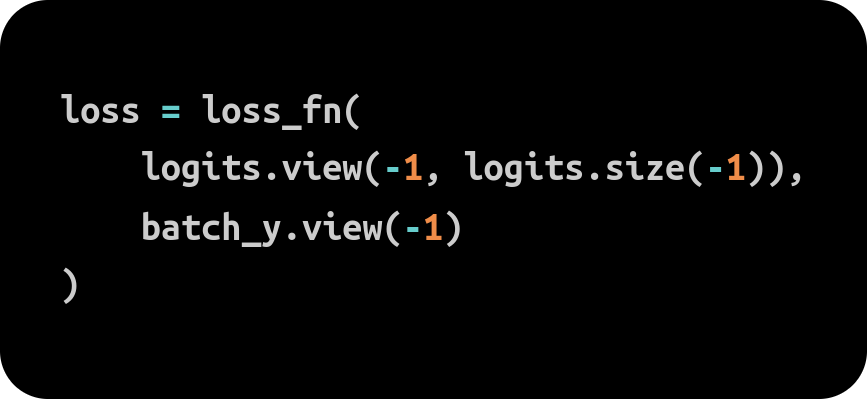
\includegraphics[width=0.5\linewidth]{img/cross_entropy.png}
    \caption{Función de pérdida del modelo \parencite{geeksforgeeks_crossentropy}}
    \label{fig:placeholder20}
\end{figure}

Dado que la función \texttt{CrossEntropyLoss} recibe como entrada dos tensores, uno con las predicciones del modelo (\textit{logits}) y otro con las etiquetas reales, sus dimensiones deben ajustarse al formato esperado. El primer tensor debe tener forma \texttt{[N, C]}, donde \texttt{N} representa el número total de tokens que el modelo intenta predecir y \texttt{C} corresponde al número de posibles tokens del vocabulario. El segundo tensor debe tener forma \texttt{[N]}, conteniendo para cada posición el índice del token correcto. Por ello, los tensores se aplanan mediante \texttt{.view(-1, logits.size(-1))} para los \textit{logits} y \texttt{.view(-1)} para las etiquetas reales.

A través de esta función de pérdida, se calcula la perplejidad \parencite{keerthanams2025evaluating}, que mide la incertidumbre al predecir la siguiente palabra. Por ejemplo, una perplejidad de 10 indica el modelo, en promedio, es tan incierto como si tuviera que elegir uniformemente entre 10 opciones. Matemáticamente, se define como:
\[
\text{PPL} = e^{\mathcal{L}_{CE}}
\]

Una perplejidad baja indica que el modelo es bueno prediciendo la siguiente palabra, mientras que una alta sugiere que el modelo está confundido. Durante el entrenamiento, se monitoriza la perplejidad en los conjuntos de validación para evaluar el progreso del modelo y ajustar hiperparámetros si es necesario.

\begin{figure}[h]
    \centering´
    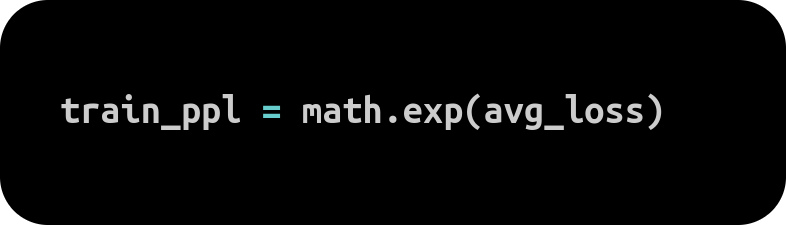
\includegraphics[width=0.5\linewidth]{img/perplexity.png}
    \caption{Calculo de perplejidad en PyTorch \parencite{stackoverflow_perplexity_pytorch}}
    \label{fig:placeholder21}
\end{figure}

El problema de la perplejidad \parencite{singh2024perplexitymatters} es que depende altamante del vocabulario, con lo que puede llegar a darse que un modelo bueno parezca malo debido a palabras poco comunes en vocabularios extensos. En este caso, el vocabulario no es muy extenso y al usar \texttt{BPE} se reduce el nñumero de palabras poco comunes o desconocidas, con lo que se ha considerado una métrica adecuada. Por otro lado, no valida la corrección semántica o contextual, por lo que a la hora de validar el modelo se han planteado otras técnicas como \texttt{MAUVE} \parencite{krishnap25_mauve_github} (ver sección \ref{sec:mauve} del Anexo) y \texttt{Distinct-n} (ver sección \ref{sec:distinct-n} del Anexo), además de la validación humana configurando la temperatura, como se explicará en la sección \ref{subsec:validacion}.

Por último, se ha implementado un mencanismo del tipo \textit{Early Stopping} por el cual si la perplejidad en los datos de validación no mejora durante un periodo consecutivo se finaliza el entrenamiento. Con esto se pretende evitar sobreajuste y que el modelo se ajuste demasiado bien a los datos de entrenamiento respecto a los de validación.

\begin{figure}[h]
    \centering´
    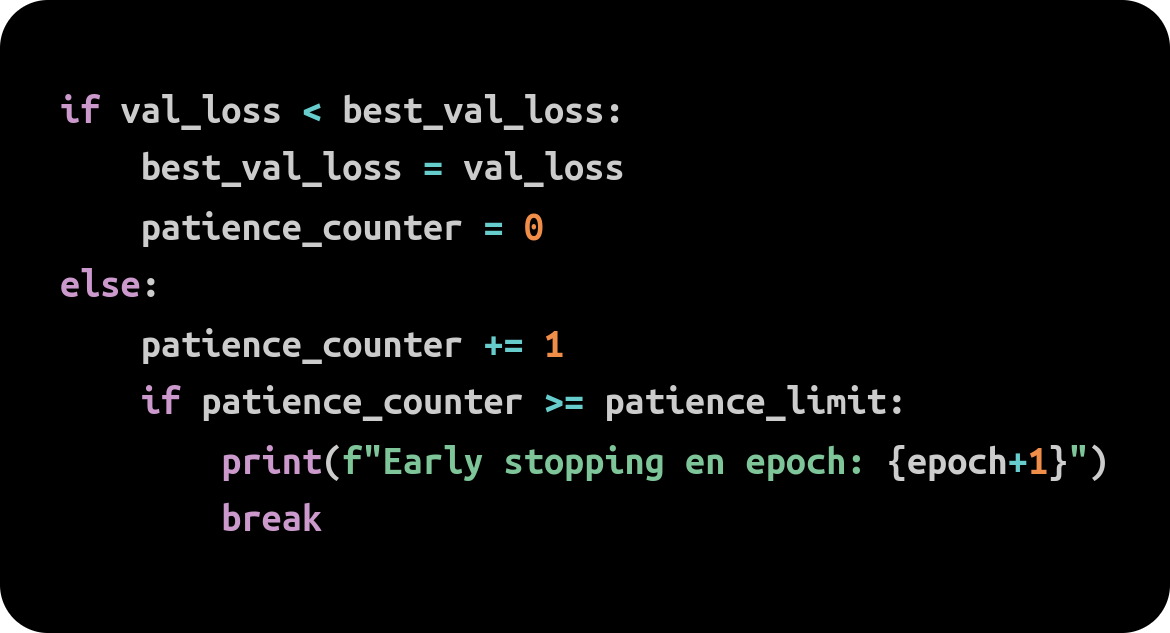
\includegraphics[width=0.5\linewidth]{img/early_stop.png}
    \caption{Calculo de perplejidad en PyTorch \parencite{stackoverflow_perplexity_pytorch}}
    \label{fig:placeholder23}
\end{figure}

\subsection{Optimizadores}

Se han probado 3 optimizadores distintos, pero a la vez altamente relacionados. En primer lugar el optimizador Stochastic Gradient Descent (SGD), quien introdujo un cambio respecto al tradicional descenso del gradiente, y es que el gradiente no se calcula sobre todo el conjunto de datos original, sino sobre una muestra aleatoria del conjunto de entrenamiento \parencite{geeksforgeeks_sgd}. Ciertas investigaciones indican que pese a utilizar un ratio de aprendizaje constante, lo que puede ocasionar una convergencia lenta, generaliza mejor que Adam y es buento evitando el sobreajuste \parencite{ultralytics_adam_glossary}. 

Otro de los optimizadores es Root Mean Square Propagation (RMSProp). Este optimizador mejora su rendimiento para funciones de pérdida no convexas, ajustando el ratio de aprendizaje, dado que un solo valor no funciona igual de bien para cada parámetro, haciendo que algunos pesos apenas cambien y otros cambien demasiado. Da estabilidad \parencite{kashyap2024rmsprop}.

Por último, se ha utilizado AdamW. Es un optimizador utilizado en GPT por su alta capacidad de generalización . Se diferencia de Adam en que desacopla el decaimiento del peso \textit{weight decay}, una regularización que castiga pesos grandes para evitar sobreajustes, del proceso de actualización del gradiente \parencite{datacamp_adamw_pytorch}.  Al igual que Adam, se basa en dos operaciones \parencite{yassin2024adamvsadamw}, por un lado el impulso o \textit{momentum}, y por otro lado el uso de un \textit{learning rate} adaptativo. El primer factor implica que no solo se considere el punto actual en cada paso durante el descenso por gradiente, si no que considera los pasados, así, se logran movimientos más suaves y un descenso más rápido y estable. El segundo factor hace que los ratios de aprendizaje se ajusten en base a los gradientes de los parámetros (RMSProp).

La implementación es muy simple y la dificultad reside más en ajustar los hiperparámetros. En el caso de AdamW se han seguido las recomendaciones dadas en \parencite{datacamp_adamw_pytorch}, que indica partir con un \textit{learning rate} de $10^-3"$ y un \textit{weight decay} de $10^-2"$ a $10^-4"$, siendo mayor para modelos más complejos. 


\begin{figure}[h]
    \centering´
    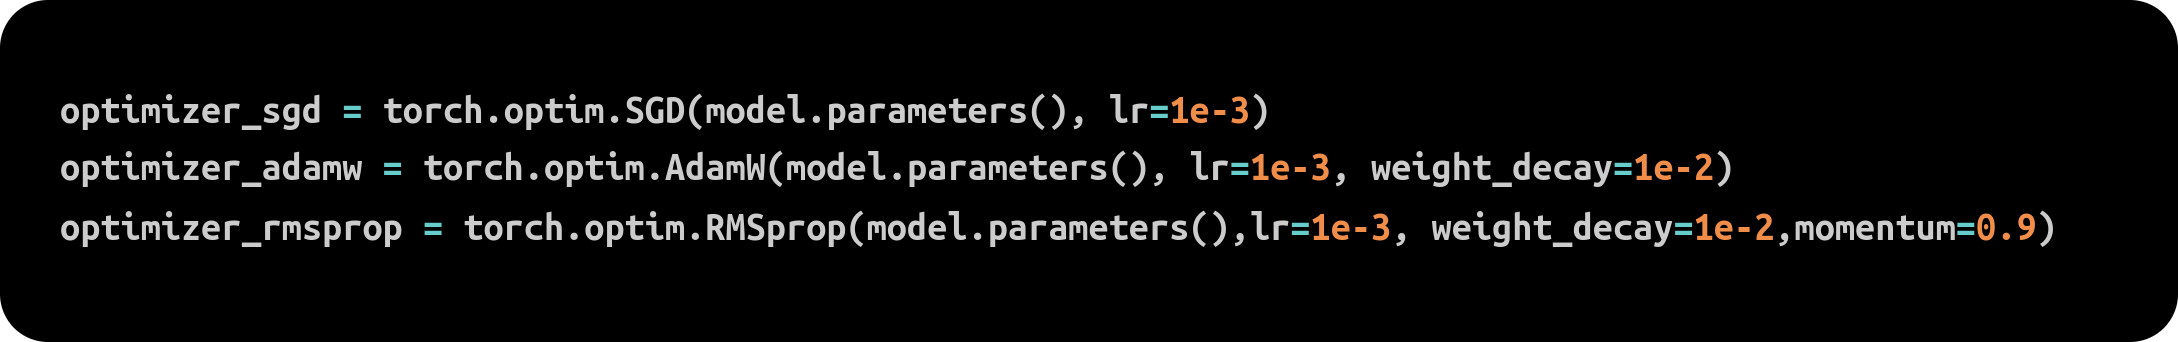
\includegraphics[width=0.5\linewidth]{img/optimizers.png}
    \caption{Optimizadores \parencite{stackoverflow_sgd_optimizer}}
    \label{fig:placeholder22}
\end{figure}


\subsection{Resumen del modelo para Tiny Shakespeare}

En primer lugar se tokeniza el dataset de entrenamiento, que contiene $896.135$ caracteres. Para ello se utiliza un tokenizador \textit{BPE} a través de \textit{SentencePiece}, que es entrenado con estos datos y aprende una reglas de segmentación y un vocabulario. A través de este tokenizador ya entrenado, se tokenizan los datos de entrenamiento, validación y test. Como el tamaño definido para el vocabulario es de $16000$ elementos, se obtiene un conjunto de números enteros que representan valores (índices) dentro de ese vocabulario con valores comprendidos entre $0$ y $15999$. En total se generan $265566$ índices para el dataset de entrenamiento. 

La función del modelo es dado cada token, predecir el siguiente. Es por ello que un paso previo a transformar este vector a embeddings se crea un dataset de \texttt{PyTorch} que, junto con \textit{DataLoader} genera ejemplos de secuencias de entrada y objetivos (se desplaza una posición la de entrada) y se agrupan en batches, que irán alimentando las capas de Embedding del modelo. Aquí cabe resaltar que, como el tamaño del batch es de $64$, el modelo recibe como entrada tensores con tamaño $(64,256)$. Para verlo mejor, es como si el modelo recibe: \textit{[El, perro, ladra, en, el]} y busca predecir \textit{[perro, ladra, en, el,prado]}, para cada token.


Cada uno de estos batch alimentan el modelo durante $20$ épocas. En primer lugar entran a las capas de embedding. Aquí los vectores de tamaño $(64,256)$ se convierten a vectores multidimensionales (embeddings) de tamaño $(64,256, 512)$, es decir, cada token, se convierte en un vector de $512$ elementos, y son sumados al \textit{Positional Embedding} para que el modelo sea consciente de la posición de cada token en la secuencia. 

Tras esto, los embeddings avanzan a los bloques principales de la arquitectura, que se replican $6$ veces. Estos, son los bloques de atención con máscara causal y 8 cabezas, las capas de normalización y adicción y Feed Forward, quien expande la entrada de tamaño $(64,256, 512)$ para añadir no linealidad y la vuelve a comprimir a su tamaño inicial. Estos bloques se apilan a través de \texttt{nn.ModuleList}. 

Finalmente, tras salir del bloque principal, la salida pasa de nuevo por una capa de normalización y finalmente se obtienen los \textit{logits} gracias a una capa lineal. 

El proceso se repite el número de épocas mencionado y se valida con datos de validación y \textit{CrossEntropy}, utilizando la perplejidad para determinar si el modelo aprende o no.


\subsection{Validación} \label{subsec:validacion}





%--- FIN DEL CAPÍTULO 4

\clearemptydoublepage

%--- CAPÍTULO 5 DEL TFM
\chapter{Conclusiones}

\section{Primera aproximación con Tiny Shakespeare}

Se ha realizado un primer entrenamiento con $20$ épocas y un \textit{Early Stopping} con paciencia igual a 10. El optimizador utilizado es \texttt{AdamW} con un ratio de aprendizaje de $1.5*10^-3$ y \textit{weight decay} igual a $0.01$. Además se ha aplicado \texttt{CosineAnnealingLR} para ir ajustando durante el entrenamiento el ratio de aprendizaje, no solo a nivel de época, sino de batch. El resto de parámetros del modelo son: 

\begin{itemize}
    \item \textbf{Tamaño vocabulario}: $10000$
    \item \textbf{Tamaño embedding}: $512$
    \item \textbf{Tamaño contexto}: $256$
    \item \textbf{Tamaño de batches}: $64$
    \item \textbf{Tamaño FFNN}: $1024$
    \item \textbf{Número de batches por época}: $4146$
    \item \textbf{Número de cabezas de atención}: $8$
    \item \textbf{Número de capas}: $6$
    \item \textbf{Dropout}: $0.1$
\end{itemize}

Con ello, se han entrenado $11$ épocas antes del \textit{Early Stopping}, comenzando en la primera época con una pérdida de $6.23$ y una perplejidad de  $509.94$ para datos de entrenamiento y de $586.34$, para datos de validación y finalizando con una périda de $6.2226$ y perplejidad de $504.00$ y $598.18$ respectivamente. Se ve un descenso en los datos de entrenamiento, frente a un incremento en validación lo que suscita un sobreajuste, además no se aprecia un cambio significativo de los valores a lo largo de las épocas lo que hace intuir que el modelo no está aprendiendo nada significativo.

\begin{figure}[h]
    \centering´
    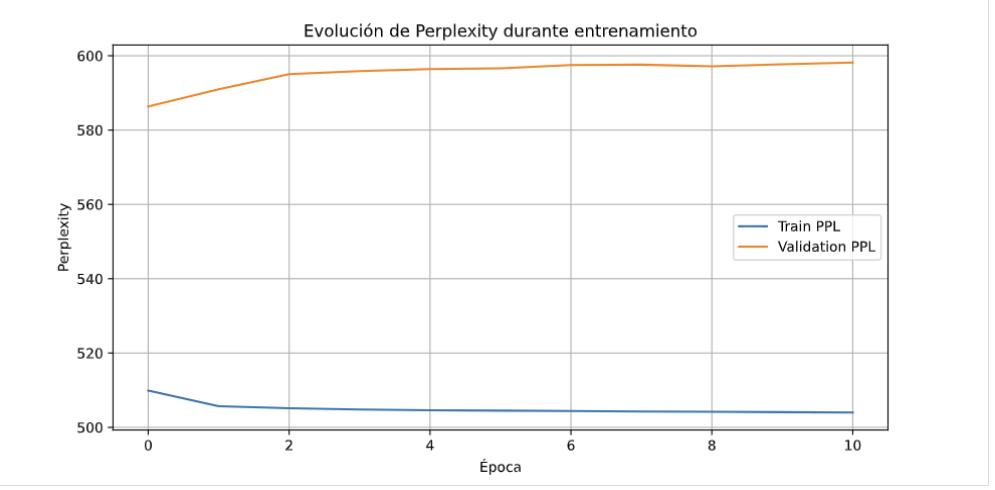
\includegraphics[width=0.5\linewidth]{img/resultado_entrenamiento_v1.png}
    \caption{Resultado primer entrenamiento}
    \label{fig:placeholder24}
\end{figure}

Para corregirlo se ha reducido el tamaño del vocabulario y el modelo, pues al ser un dataset pequeño, sin gran dispersión, se ha visto que esto da mejores resultados. Además, se ha ajustado el optimizador incluyendo como coeficientes de decaimiento exponencial los valores $0.9$ y $0.98$ \parencite{reddit_transformer_not_learning}. Para evitar divisiones por cero en el cálculo de los momentos, se ha añadido un valor $\epsilon$ igual a $10^-9$. A esto se ha añadido un \textit{scheduler} basado en la clase LambdaLR de PyTorch \parencite{pytorch_adjust_lr}, el cual permite modificar dinámicamente la tasa de aprendizaje en función del número de pasos de entrenamiento. En este caso, se ha definido una función que implementa una fase de warm-up de $1000$ iteraciones, durante la cual la tasa de aprendizaje aumenta linealmente desde 0 hasta su valor máximo inicial. Este procedimiento ayuda a estabilizar el entrenamiento en las primeras etapas, evitando actualizaciones abruptas de los parámetros cuando el modelo todavía no ha alcanzado una representación estable de los gradientes. Por último, otro cambio que se ha llevado a cabo ha sido cambiar el modo de normalización. Se estaba haciendo lo que se conoce como \texttt{Post-normalización}, es decir, la normalización se aplica después de cada subcapa (atención y feed-forward). Sin embargo, ciertos estudios sugieren que la \texttt{Pre-normalización}, donde la normalización se aplica antes de cada subcapa, puede mejorar la estabilidad del entrenamiento \parencite{doherty2024_hownot}.

Los nuevos parámetros del modelo son:
\begin{itemize}
    \item \textbf{Tamaño vocabulario}: $8000$
    \item \textbf{Tamaño embedding}: $256$
    \item \textbf{Tamaño contexto}: $128$
    \item \textbf{Tamaño de batches}: $64$
    \item \textbf{Tamaño FFNN}: $1024$
    \item \textbf{Número de batches por época}: $4146$
    \item \textbf{Número de cabezas de atención}: $8$
    \item \textbf{Número de capas}: $3$
    \item \textbf{Dropout}: $0.3$
\end{itemize}
Con ello, manteniendo el \textit{Early Stopping} se ha logrado un decaimiento progresivo del modelo en $40$ épocas, sin aparecer sobreajuste, obteniendo una pérdida de $3.8240$ y una perplejidad de $91.41$ en datos de validación y $45.79$ en entrenamiento. En la imagen \ref{fig:placeholder25} se ven mejor los resultados.


\begin{figure}[h]
    \centering´
    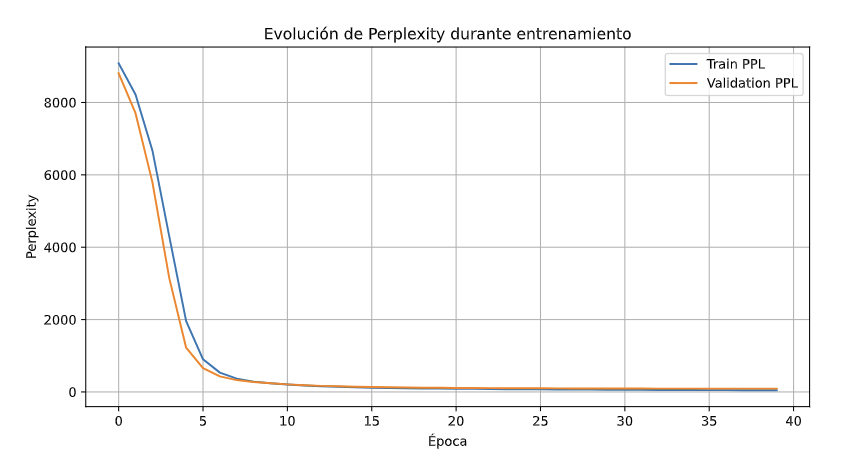
\includegraphics[width=0.5\linewidth]{img/resultado_entrenamiento_v2.png}
    \caption{Resultado primer entrenamiento}
    \label{fig:placeholder25}
\end{figure}

\section{Validación}
Para validar se utiliza el conjunto de datos reservados para tal fin ($35327$ tokens), los cuales no han sido vistos por el modelo durante el entrenamiento. Se obtiene una pérdida de $4.5039$ y una perplejidad de $90.37$, de media para un total de 550 lotes. Es buena señal pues indica que el modelo ha aprendido patrones generales y no se ha sobreajustado a los datos de entrenamiento.

Además de una validación con el conjunto de test, se ha implementado un método que consta de distintos hioerparámetros ajustables para generar texto a partir de unos tokens dados, como por ejemplo: "King Charles". Estos hiperparámetros son los siguientes \parencite{vyas2025transformer_decoder_part3}: 

\begin{itemize}
    \item Temperatura.
La temperatura ajusta la aleatoriedad en las respuestas del modelo al generar texto. Una temperatura baja hace que el modelo sea más determinista, eligiendo las palabras con mayor probabilidad, lo que puede resultar en respuestas repetitivas o predecibles. Por otro lado, una temperatura alta introduce más aleatoriedad, permitiendo al modelo explorar opciones menos probables y generando respuestas más variadas y creativas. En sí lo que hace es escalar los logits antes de calcular la distribución de probabilidades con la función \textit{softmax} del siguiente token. Matemáticamente, se expresa como:
    \[
        P(z_i) = \frac{e^{(z_i / T)}}{\sum_{j} e^{(w_j/ T)}}
    \]
Donde cada $z_i$ es un logit. Aquí a la hora de implementarlo se ha decidido que si la temperatura es $0.0$, no se aplica ninguna transformación, pues investigando he visto que se trataría como \textit{argmax}, es decir, siempre se elegiría la palabra con mayor probabilidad \parencite{vishnuraj2025temperature}.

    \item Top-k.
En lugar de escoger siempre el token con mayor probabilidad, lo que introduce respuestas repetitivas y poco naturales, con este método se seleccionan los \textit{k} tokens más probables y se normalizan sus probabilidades. Luego, se elige aleatoriamente entre estos \textit{k} tokens, lo que permite al modelo generar respuestas más variadas y creativas. La implementación se hace a través del método de \texttt{PyTorch} \textit{topk}, que devuelve los \textit{k} valores más altos de un tensor junto con sus índices. En este caso, se utiliza para filtrar los logits, manteniendo solo los \textit{k} más altos y estableciendo el resto a $-\infty$, lo que hace que su probabilidad sea prácticamente nula tras aplicar la función \textit{softmax}.

    \item Top-p (Núcleo de muestreo).
Se trata de otro método similar a Top-k. En este caso se ordenan los tokens por probabilidad hasta que la suma acumulada sea mayor o igual a un umbral \textit{p}. Luego, se normalizan las probabilidades de estos tokens seleccionados y se elige aleatoriamente entre ellos. Para la implementación, al igual que ocurre con el método anterior se ha seguido el ejemplo dado en \parencite{bsantraigi_topk_topp_batched}. En primer lugar se ordenan los logits de mayor a menor, a continuación, se calcula la suma acumulada de las probabilidades tras aplicar \textit{softmax} mediante la función \textit{cumsum}. Finalmente, se filtran los logits, estableciendo a $-\infty$ aquellos cuya suma acumulada supere el umbral \textit{p}, lo que hace que su probabilidad sea prácticamente nula tras aplicar la función \textit{softmax}.

    \item Número máximo de tokens a generar. Se establece un máximo número de tokens a generar para evitar que crezca indefinidamente la respuesta.
    
    \item Presence y frequency penalty \parencite{vyas2025transformer_decoder_part3}.
Se trata de dos métodos para reduucir o evitar la repetición de frases o tokens previos. El primero penaliza en base a si ha aparecido o no un token previamente y el segundo se basa en el número de veces que ha aparecido. Matemáticamente se expresa como: 
    \[
        z_i = z_i(w) - \text{presence\_penalty} \cdot \alpha - \text{frequency\_penalty} \cdot \beta
    \]

    donde $\alpha$ y $\beta$ son los coeficientes de penalización para presencia y frecuencia respectivamente.
A la hora de implementarlo se calcula esa expresión con tensores, $\alpha$ es un tensor binario que indica si el token ha aparecido o no y $\beta$ es un tensor con el número de veces que ha aparecido cada token obtenido a través del método \textit{bincount} que cuenta el número de ocurrencias de cada valor en un tensor de enteros no negativo.

\subsection{Resultados}

Se ha probado a generar texto con distintas combinaciones, partiendo de unos mismos tokens iniciales: \textit{"KING RICHARD:"} y un número máximo de tokens a generar igual a $100$. En la tabla \ref{tab:resultados_validación_shakespeare} se muestran los resultados.
\begin{table}[h!]
    \centering
    \caption{Hiperparámetros}
    \label{tab:resultados_validación_shakespeare}
    \begin{tabular}{cccccc}
    \toprule
    \textbf{Temperatura} & \textbf{Top-k} & \textbf{Top-p} & \textbf{Presence Penalty} & \textbf{Frequency Penalty} & \textbf{Resultado}  \\
    \midrule
    0.2 & 50 & 0.90 & 0.0 & 0.0 \\
    0.5 & 100 & 0.95 & 0.2 & 0.1 \\
    0.8 & 150 & 0.98 & 0.5 & 0.3 \\
    1.0 & 200 & 1.00 & 1.0 & 0.5 \\
    \bottomrule
\end{tabular}
\end{table}

\end{itemize}

%-------------------------------
%--- FIN DEL CAPÍTULO 5

\clearemptydoublepage

\printbibliography[title={Referencias Bibliográficas}]

\appendix 
\chapter{Anexos}

\section{GELU} \label{sec:gelu}
\section{Xavier Uniform} \label{sec:xavier}
\section{Normal uniform} \label{sec:normal}

\section{Entropía} \label{sec:entropia}

\section{MAUVE} \label{sec:mauve}


\section{Distinct-n} \label{sec:distinct-n}

%--- FIN DE ANEXOS

\clearemptydoublepage

\end{document}





https://discuss.pytorch.org/t/how-to-use-collate-fn/27181
https://plainenglish.io/blog/understanding-collate-fn-in-pytorch-f9d1742647d3
https://blog.lukesalamone.com/posts/custom-pytorch-collate/

https://www.kaggle.com/code/shreydan/bpe-tokenizer-lstm-embeddings -> IMplementación
\begin{lstlisting}[language=Python]

for batch_x, batch_y in loader:
    B, T = shape(batch_x)

    # Embeddings
    tok = TokenEmbedding(batch_x)                # [B, T, D]
    pos_ids = arange(T).expand(B, T)             # [B, T]
    pos = PosEmbedding(pos_ids)                  # [B, T, D]
    x = tok + pos                                # [B, T, D]

    # Repite N veces (capas del decoder)
    for layer in 1..N:
        # (Pre-Norm) Self-Attention enmascarada
        a = SelfAttention( LayerNorm(x), mask=causal(T) )   # [B, T, D]
        x = x + a                                           # residual

        # (Pre-Norm) Feed-Forward
        f = FeedForward( LayerNorm(x) )                     # [B, T, D]
        x = x + f                                           # residual

    # Proyección a vocabulario
    logits = Linear(x)                           # [B, T, vocab_size]

    # Pérdida (teacher forcing: batch_y es x desplazado +1)
    loss = CrossEntropy( logits.view(-1, vocab_size),
                         batch_y.view(-1) )

    optimizer.zero_grad()
    loss.backward()
    optimizer.step()


for batch_x, batch_y in loader:
    tok_emb = embedding_layer(batch_x)                      # [B,T,D]
    pos_ids = arange(T).expand(B,T)
    pos_emb = pos_embedding_layer(pos_ids)                  # [B,T,D]
    x = tok_emb + pos_emb

    for _ in range(N):
        x = x + masked_multihead_self_attention( layer_norm(x) )
        x = x + feed_forward( layer_norm(x) )

    logits = linear(x)                                      # [B,T,V]
    loss = cross_entropy( logits.view(-1,V), batch_y.view(-1) )
    optimizer.zero_grad(); loss.backward(); optimizer.step()


    
\end{lstlisting}